\documentclass[a4paper, 12pt]{article}
\usepackage{outlines}
\usepackage{graphicx}
%\usepackage{times}
\usepackage{xcolor}
\usepackage{float}
\usepackage{mathtools}
\usepackage{enumerate}
\usepackage{geometry}
\usepackage[english]{babel}
\usepackage{array}
\usepackage{wrapfig}
\usepackage{amsmath}
\usepackage{multirow}
\usepackage{tabu}
\usepackage{titlesec}
\usepackage{titletoc}
\usepackage{array}
\usepackage{tabularx,ragged2e,booktabs,caption}
\usepackage{chngcntr}
\usepackage{pgf-pie}  
\counterwithin{figure}{section}
\counterwithin{table}{section}
\usepackage{colortbl}

\titleformat{\section}[display]%
{\null\fontsize{16}{5}\rmfamily\bfseries\filcenter}{CAPITOLUL \thesection}{1em}{}[]
\titleformat{name = \section, numberless}[block]%
{\null\fontsize{16}{5}\rmfamily\bfseries\filcenter}{}{1em}{}
\titlespacing*{\section}{0em}{1em}{1em}

\titlecontents{section}
[7em] % ie, width of contentslabel + 0.5em
{\medskip}
{\contentslabel[\MakeUppercase\chaptername~\thecontentslabel]{7.5em}}%\thecontentslabel
{\hspace*{-6.5em}}
{\titlerule*[0.5pc]{.}\contentspage}

\addto{\captionsenglish}{
	\renewcommand{\refname}{Referințe bibliografice}%
	\renewcommand{\contentsname}{Cuprins}
	\renewcommand{\listfigurename}{Lista imaginilor}
	\renewcommand{\listtablename}{Lista tabelelor}
}
\addto\captionsenglish{\renewcommand{\chaptername}{Capitolul}}
%define the page geometry
\geometry{
	a4paper,
	left=25mm,
	top=25mm,
	bottom=25mm,
	right=25mm,
}
\renewcommand{\baselinestretch}{1.5}
\makeatletter
\renewcommand\paragraph{\@startsection{paragraph}{4}{\z@}%
	{-2.5ex\@plus -1ex \@minus -.25ex}%
	{1.25ex \@plus .25ex}%
	{\normalfont\normalsize\bfseries}}
\makeatother
\setcounter{secnumdepth}{4} % how many sectioning levels to assign numbers to
\setcounter{tocdepth}{4}    % how many sectioning levels to show in ToC



\begin{document}

%define the title page
\begin{titlepage}
	\begin{center}
		\vspace{0.5cm}
		\LARGE \textsc{Universitatea "Babeș Bolyai"}
		\LARGE \textsc{Cluj-Napoca}
		\\
		\vspace{0.5cm}
		\Large \textsc{Facultatea de studii europene}
		\\
		\Large \textsc{Specializare Management}
		
		
		\vspace{1.5cm}
		
		\Huge Comportamentul consumatorului online roman tanar si educat - Studiu de caz
		\\
		\bigskip
	

		\vspace{0.5cm}		
		\Large LUCRARE DE LICENȚĂ
		
		\vfill
		
		\Large
		\textsc{Coordonator}\hfill \textsc{Autor}
		\\
		\large
		\textsc{Conf. dr. Nicoleta RACOLȚA-PAINA}\hfill\textsc{CIUCANU Elena- Sorina}
		
		\vspace{1.5cm}
		\textsc{Cluj-Napoca, România}\\
		\textsc{Iulie 2021}
		
	\end{center}
\end{titlepage}
\restoregeometry

%put the table of contents
\tableofcontents

%put the list of figures
\newpage
\listoffigures
\newpage
\listoftables

%this section is on new page
\newpage
\nocite{bobalcua2015loyal}
\nocite{london_economics_2011}
\nocite{duralia2016particularities}
\nocite{devderea2018consumer}
\nocite{armstrong2014principles}
\nocite{orzan2014study}
\nocite{obradattitudes}
\nocite{sava_2020}
\nocite{bighiu2015compulsive}
\nocite{gorunescu_2020}

\section*{Declaratie}
\newpage

	\section*{Introducere}
\addcontentsline{toc}{section}{\textsc{Introducere}}
	
	\quad\quad Lucrarea de față, "Comportamentul consumatorului online român, tânăr și educat- Studiu de caz" abordează un subiect vast și de actualitate, care devine din ce în ce mai important pentru firmele care doresc să-și dezvolte strategii de marketing axate pe factorii ce determină consumatorul online să aleagă un producător în detrimentul altuia. Numărul de studii publice pe tema procesului de cumpărare a consumatorului online din România este mic comparativ cu numărul de articole din alte țări, atât din Uniunea Europeană cât și din afară acesteia. Dorim să precizăm că această lucrare pune accentul pe consumatorul  individual și nu pe cel organizațional (entități juridice) deoarece dorim să analizăm ce anume determină cumpărătorul individual să achiziționeze produse care sunt de larg consum.
	
	\quad Scopul prezentei lucrări de licență este realizarea unui profil al consumatorului online tânăr și educat din România pentru ca firmele din comerțul electronic să înțeleagă mai bine comportamentul acestuia și să se plieze pe nevoile și dorințele lui.
	
	\quad Prezentul studiu își propune să prezinte principalele aspecte teoretice cu privire la comportamentul consumatorilor online, respectiv practice referitoarea la factorii care influențează comportamentul consumatorului online român,tânăr și educat, pentru ca în final să oferim informații de folos companiilor ce practică comerțul electronic și sunt prezente pe piața din România.
	
	\quad La fel ca orice demers științific, este nevoie de existența unei baze teoretice care să vină în ajutorul analizei informațiilor obținute în urma studiului de caz. Astfel, pentru partea teoretică este utilizată cartea fondatorului marketing-ului, Philip Koetler, articole de la Comisia Europeană, privind la nivel de Uniune consumatorul online, dar și câteva articole de la autori români precum Duralia Oana de la Universitatea Lucian Blaga din Sibiu și Claudia Bobâlcă care și-au manifestat interesul față de percepția consumatorilor online, tineri asupra bunurilor online. 
	
	\quad Partea practică reprezintă o cercetare primară cantitativă, metoda folosită fiind sondajul de opinie, iar instrumentul de culegere a datelor fiind chestionarul (lansat online în perioada 27.04.-04.05) . Chestionarul folosit (vezi Anexa 1) cuprinde 3 întrebări filtru și anume una legată de vârstă( intervalul țintit de noi fiind 18-30 ani), o altă întrebare legată de nivelul de studii (minim BAC) și respectiv numărul de achiziții online, cu plata card în februarie-aprilie 2021 (aici dorind să avem răspunsuri de la consumatorii avizați). Am ales că respondenții să aibă un anumit interval de vârstă și anume 18-30 deoarece în domeniul marketing-ului este necesară poziționarea și segmentarea pieței țintă.
	
	\quad Structura lucrării include atât o secțiune teoretică cât și o secțiune practică, având în total un număr de 4 capitole. Primul capitol, numit "Comportamentul consumatorului online - conținut și tendințe" cuprinde 6 subcapitole dar și subsubcapitole în care se discuta la modul general de consumatorul online. Astfel, prima parte a capitolului cuprinde o introducere a subiectului și anumite bariere ce se regăsesc în mediul digital. Pe urmă, lucrarea pune accent pe consumatorul online începând cu importantă comportamentului consumatorului,  managementul relațiilor cu clienții - metodă folosită astăzi de companii pentru a-și loializa clienții, tipuri de decizii pe care consumatorii obișnuiesc să le facă, apoi cu trend-uri prezente în cererea cumpărătorilor, modele de marketing care fac legătură dintre tehnologie și consumatorul online, urmând apoi o scurtă comparație cu diferențe și asemănări între mediul online și offline. Capitolul continuă cu factorii care tind să influențeze decizia de cumpărare a acestuia, procesul de cumpărare împărțit și detaliat pe etape și în cele din urmă,  beneficiile și provocările pe care consumatorii online le-au întâlnit și depășit în experiențele lor în mediul online. 
	
	\quad Al doilea capitol, numit "Cercetare secundară privind comportamentul constumatorului online, tânăr și educat din România" cuprinde 4 subcapitole. Primul subcapitol relevă informații despre comerțul electronic din România oferind statistici despre cumpărăturilor online ale românilor, categoriile de produse care sunt cumpărate cel mai frecvent, online, de populația din România și contextul actual al pandemiei Covid19 care a avut o influență puternică asupra achizițiilor online. Următoarele subcapitole includ trei perspective asupra achizițiilor online din România, articole ce oferă informații despre comportamentul consumatorului online, tânăr și educat din România, iar la final o scurtă concluzie a celor trei articole.
	
	\quad Lucrarea continuă cu al treilea capitol, care cuprinde cercetarea propriu-zisă și reprezintă esența prezenței lucrări științifice deoarece realizează conexiunea între elementele teoretice cuprinse în capitolele anterioare și modul în care se aplică acestea în practică. Astfel, după cum am menționat anterior, în elaborarea acestui capitol este utilizat o metodă de cercetare cantitativă (instrumentul folosit fiind chestionarul) pentru a obține informațiile necesare atingerii obiectivelor propuse și anume, crearea unui profil al consumatorului online, tânăr și educat din România.
	
	\quad Lucrarea prezintă o serie de limite ca urmare a lipsei surselor bibliografice și studiilor datorat numărului scăzut de cercetări asupra comportamentului consumatorului online, tânăr și educat din România. De asemenea, reticiența respondenților de a răspunde la chestionar, în special a respondenților de genul masculin, mi-a îngreunat munca în cercetarea mea cantitativă. Un aspect neașteptat a fost numărul mare de respondenți care au ales la întrebarea filtru, referitoare la numărul minim de achiziții online în perioada februarie-aprilie 2021, mai puțin de 5 achiziții online, fapt ce m-a determinat să nu includ in cercetarea mea o mare parte din totalul de respondenți.
	
	\quad Luând în considerare cele afirmate mai sus, exprimăm speranța că această cercetare aduce un plus de valoare pentru domeniul teoretic, referitor la comportamentul consumatorului online, tânăr și educat din România și implicarea sa în comerțul electronic.
		
	\newpage
	\setcounter{section}{0}
	\section{Comportamentul consumatorului online - conținut și tendințe}
	
	\quad\quad Societatea în care trăim se află într-o continuă stare de schimbare. Ultimii ani de evoluție în domeniul comunicației, tehnologiei, informației și marketingului au creat noi schimbări în modul în care consumatorii se informează și cumpără anumite produse și servicii. În acest capitol se discută despre nouă modalitate, folosită în marketing, pentru a facilita schimbul de produse dintre cumpărător și producător, prin intermediul internetului, și anume, comerțul electronic. Apoi, se analizează comportamentul consumatorului fizic și online prin prisma a mai multor concepte și procese ce ne ajuta sa intelegem gandirea si comportamentului acestuia. 

		\subsection{Comertul electronic}
	\quad \quad\space În ultimii zece ani, în contextul internațional al comunicării digitale, comerțul electronic devine o importantă parte a sistemului de afaceri. Odată ce Internetul a devenit un instrument foarte utilizat și important în comunicare, promovare și tranzacții comerciale, noi platforme s-au dezvoltat pentru a crea strategii competitive.
	
	\quad Diverse articole susțin faptul că comercializarea produselor este încă necesară și vitală, însă nu mai este suficientă pentru ca o companie să-și păstreze poziția pe piață. Astfel s-a introdus un nou concept numit experiența clienților, definit drept "răspunsul intern și subiectiv pe care îl au clienții la orice contact cu o companie", pentru a descrie noua relație dintre brand-uri și clienți.\footnote{Mihaela Știr, "Business to consumer- Ecommerce in România-Evolution and trends", 2019, p.128} Noile așteptări ale consumatorilor moderni sunt influențate de schimbările tehnologice care au afectat structurile comerciale, crescând interesul consumatorilor pentru E-commerce. Că să putem fi mai clari, vom defini comerțul electronic drept "orice formă de tranzacție comercială unde părțile implicate interacționeaza într-un mod electronic".\footnote{Claudia Bobalca, "The Loyal Customers’ Perception Regarding The Online Buying Process", \textit{Central and Eastern European Online Library}, Economie, p.241}	
	
	\quad Într-o economie globală, dezvoltată într-o piață foarte competitivă, orientarea spre consumator nu mai reprezintă doar un trend ci o necesitate, precum am menționat și anterior. Astfel, o bună înțelegere a modului în care consumatorii beneficiază de proprietățile Internetului și a factorilor pe care îi iau în considerare pentru a se hotăra asupra deciziilor de cumpărare în mediul comerțului electronic, aduce avantaje semnificative pentru managerii care doresc să dezvolte strategii de marketing potrivite profilului consumatorilor pe care îi au. Cumpărătorii online au acces nelimitat la informație și au oportunitatea de a alege dintr-o gama largă de opțiuni în selectarea produselor și serviciilor potrivite acestora.

	\quad În acest caz, merită remarcat faptul că comerțul electronic include ambele tipuri de tranzacții implicând atât bunuri tangibile precum electronice, bunuri de larg consum, jucării care trebuie să fie livrate fizic către consumator, dar și tranzacții privind accesul la bunuri intangibile, precum sevicii sau produse care pot fi furnizate digital către consumator. De asemenea, trebuie menționat faptul că există bunuri care se găsesc atât în format electronic cât și în format fizic precum cărțile, revistele, muzică și jocurile.

	\quad În urma experiențelor privind achiziția unor produse/servicii online, unii consumatori au întâlnit și câteva bariere care i-a determinat să evite mediul digital, printre care principalele le enumaram mai jos\footnote{European Parliament, "Consumer behaviour în a digital environment", p.77}:
	\begin{itemize}
	\item Potrivit rezultatelor de la Eurostat cel mai frecvent motiv, pe care consumatorii l-au menționat, a fost preferința pentru cumpărături în format fizic sau faptul că nu simt nevoia de a utiliza mediul online pentru a plasa comenzi.
	\item Un alt motiv foarte des întâlnit, pe care îl menționează tot informațiile de la Eurostat, sunt riscurile privind securitatea, intimitatea și grijile privind încrederea în a-și împărtăși datele personale pe care consumatorii le întâmpină atunci când doresc să plaseze o comandă online.
	\item De asemenea, consumatorii au adăugat că lipsa sau insuficiența informațiilor despre un anumit produs i-a determinat să evite achizițiile unor bunuri online.	
	\end{itemize}
\newpage
		\subsection{Comportamentul consumatorului}	
		\quad Acceptarea de către consumator a internetului drept un mijloc de informare, comparare de informații  și cumpărare a diverse bunuri și servicii a rezultat în ceea ce literatură de specialitate definește prin conceptul de e-consumator sau consumator electronic.\footnote{Oana Duralia, "Particularities of the european consumer`s behaviour în online environments", p.21}.  Spre deosebire de consumatorii tradiționali, care sunt mai conservatori și mai constanți în alegerile lor, e-consumatorii manifestă o deschidere mai mare pentru schimbare, fiind mult mai disponibili să încerce lucruri noi.\footnote{Ibidem} În plus, dacă ar fi să creăm un portret al e-consumatorului l-am putea descrie drept o persoană inovativă, creativă, educată, cu studii superioare și cu un status socio-economic ridicat.
			\subsubsection{Importanta comportamentului consumatorului }
		\quad Precum am menționat și anterior, orientarea spre consumator și cunoașterea acestuia reprezintă un element cheie al companiilor ce vor să-și crească vânzările și să-și loializeze clienții. Astfel, este importantă identificarea și analiza comportamentului cumpărătorului pentru a obține succesul pe piață..
		
		\quad În articole și cărți există diverse definiții pentru comportamentul consumatorului. Conform Asociației de marketing din America comportamentul consumatorului este definit că: \textit{"interacțiunea dinamică a afectului și a cunoașterii, comportamentul și mediul prin care ființele umane desfășoară aspectele de schimb ale vieții lor"}. Alți autori definesc comportamentul consumatorului că fiind \textit{"studiul tuturor proceselor implicate în activitatea indivizilor sau grupurilor de indivizi care aleg, cumpără, utilizează sau elimină produsele, servicii sau idei care duc la satisfacerea nevoilor sau dorințelor consumatorilor"}. Specialiștii în marketing din România au convenit asupra unei definiții clare a conceptului de comportament al consumatorului că fiind: \textit{"toate actele decizionale ale individului sau ale grupului, legate direct de obținerea și utilizarea produselor și serviciilor, pentru a satisface nevoile prezente și viitoare, inclusiv toate procesele decizionale care preced și determină aceste acte"}.\footnote{Dumitrescu Luigi, Orzan Gheorghe, Fuciu Mitrea, "UNDERSTANDING THE ONLINE CONSUMER BEHAVIOUR AND THE USAGE OF THE INTERNET AS A BUSINESS ENVIRONMENT –A MARKETING RESEARCH", 2015, p.65} 
		
		\quad Din toate definițiile menționate mai sus și, de asemenea, din multe altele, putem vedea clar un model care apare în definirea comportamentului consumatorului. Acest model conține următoarele caracteristici:\footnote{Ibidem}

		\begin{itemize}
			\item Comportamentul consumatorului se referă la indivizi, precum și la grupuri sau
			organizații;
			\item Conține întotdeauna conceptul de a satisface o anumită nevoie sau dorință,
			vremea este una personală sau organizațională;
			\item Implică întotdeauna un anumit proces care duce la decizie;
		\end{itemize}
	
			\subsubsection{Managementul relatiilor cu clientii - CRM}
		\quad Pe lângă orientarea spre consumator, care este importantă pentru menținerea avantajului competitiv și poziției pe o anumită piață, un alt element esențial îl reprezintă calitatea relației dintre un cumpărător și un producător, brand sau comerciant.
		
		\quad Acest lucru se numește, în teorie, \textbf{managementul relațiilor cu clienții - CRM}. Un astfel de sistem  urmărește informații detaliate despre clienți, astfel încât specialiștii de marketing să poată lua decizii mai orientate către clienți, care duc la relații mai durabile. Într-o orientare CRM, fiecare client reprezintă un flux potențial de resurse, mai degrabă decât o singură vânzare.\footnote{Consumer Behaviour} Astfel, conform definiției lui Koetler, am putea defini CRM drept "\textit{gestionarea informațiilor detaliate despre clienții individuali și gestionarea atentă a punctelor de contact ale clienților pentru a maximiza loialitatea clienților."}
		
		\quad În practică, atunci când un consumator cumpără aceeași marca de fiecare dată când are o nevoie pentru acel produs, se creează o relație mult mai puternică deoarece întreprinderile văd clienții fideli că fiind mult mai profitabili decât clienții care sunt predispuși la schimbarea furnizorilor de fiecare dată când fac o achiziție.  
		
		\quad\textbf{ Prin utilizarea CRM pentru a înțelege mai bine clienții, companiile pot oferi un nivel mai ridicat de servicii pentru clienți și pot dezvoltă relații mai profunde cu clienții. Ei pot folosi CRM pentru a identifica
		clienți de mare valoare, vizați-i mai eficient, vindeți încrucișat produsele companiei și creați oferte adaptate cerințelor specifice ale clienților.}
		
			\subsubsection{Tipuri de decizii}
				\quad Comportamentul de cumpărare, fie el online sau fizic, diferă foarte mult în funcție de produsul pe care consumatorul vrea să-l achiziționeze. Astfel, deciziile mai complexe implică de obicei mai mulți participanți la cumpărare și mai mulți cumpărători prudenți. În viziunea lui Koetler, există patru mari tipuri de decizii pe care consumatorul le poate lua.\footnote{Gary Armstrong, Stewart Adam, Sară Denize and Philip Koetler. Principles of marketing.2014, p.150}
			\begin{enumerate}[A)]
				\item \textbf{Comportamentul complex de cumpărare}
				
				\quad Acest tip de consumatori adoptă un comportament complex de cumpărare atunci când sunt foarte implicați într-o achiziție și percep diferențe semnificative între mărci. Consumatorii pot fi foarte implicați atunci când produsul este scump, riscant și achiziționat rar. De obicei, consumatorul are multe de învățat despre categoria de produse, însă uneori nu știe ce atribute să ia în considerare. Astfel acest cumpărător va trece printr-un proces de învățare, dezvoltând mai întâi credințe despre produs, apoi atitudini și apoi făcând o alegere de cumpărare atentă. În acest caz, comercianțîi trebuie să îi ajute pe cumpărători să învețe despre atributele clasei de produse și despre importanța lor relativă.
				
				\item \textbf{Comportamentul de cumpărare prin reducerea dezacordului}
				
				\quad Comportamentul de cumpărare care diminuează dezacordul apare atunci când consumatorii sunt foarte implicați într-o achiziție costisitoare, mai puțîn frecventă sau riscantă, dar observă diferențe mici între mărci. De exemplu, consumatorii care cumpără covoare se pot confruntă cu o decizie de implicare ridicată, deoarece covoarele sunt scumpe. Cu toate acestea, cumpărătorii pot consideră că majoritatea mărcilor de covoare dintr-o anumită gamă de prețuri sunt aceleași. În acest caz, deoarece diferențele percepute de marcă nu sunt mari, cumpărătorii pot face cumpărături pentru a află ce este disponibil, dar cumpără relativ repede. Acestea pot răspunde în primul rând la un preț bun sau la o comoditate de cumpărare.
				
				\quad După cumpărare, consumatorii ar putea experimenta dezacordul post-cumpărare (disconfort post-vânzare) atunci când observă anumite dezavantaje ale mărcii de covor achiziționate sau aud lucruri favorabile despre mărcile care nu au fost achiziționate. Pentru a contracara o astfel de disonanță, comunicările post-vânzare ale marketerului ar trebui să ofere dovezi și sprijin pentru a-i ajută pe consumatori să se simtă bine cu privire la alegerile lor de marcă.
				
				\item \textbf{Comportamentul obișnuit de cumpărare}
				
				\quad Comportamentul obișnuit de cumpărare apare în condiții de implicare scăzută a consumatorilor și a unei diferențe semnificative de marcă. Consumatorii par să aibă o implicare redusă cu cele mai ieftine produse cumpărate frecvent. În astfel de cazuri, comportamentul consumatorului nu trece prin secvența obișnuită de comportament credință-atitudine. Consumatorii nu caută pe larg informații despre mărci, nu evaluează caracteristicile mărcii și iau decizii importante despre ce mărci să cumpere.
				
				\quad Deoarece nu sunt foarte implicăți în produs, este posibil că consumatorii să nu evalueze alegerea, chiar și după cumpărare. Astfel, procesul de cumpărare implică convingeri de marcă formate prin învățare pasivă, urmat de un comportament de cumpărare, care poate fi urmat sau nu de evaluare. Deoarece cumpărătorii nu sunt foarte dedicați niciunei mărci, comercianții produselor cu implicare redusă, cu puține diferențe de marcă, utilizează adesea promoții de preț și vânzări pentru a promova cumpărarea.
				
				\item \textbf{Comportamentul de cumpărare care caută varietate}
				
				\quad Consumatorii își asumă un comportament de cumpărare în căutarea varietății în situații caracterizate prin implicare scăzută a consumatorilor, dar diferențe semnificative percepute de marcă. În astfel de cazuri, consumatorii fac multe schimbări de marcă. De exemplu, atunci când cumpără biscuiți , un consumator poate susține anumite convingeri, poate alege o marcă de biscuiți fără prea multe evaluări și apoi să evalueze marca respectivă în timpul consumului. Dar data viitoare, consumatorul ar putea alege un alt brand din plictiseală sau pur și simplu să încerce ceva diferit. Schimbarea mărcii are loc mai degrabă din motive de varietate decât din cauza nemulțumirii.
				
				\quad În astfel de categorii de produse, strategia de marketing poate diferi pentru liderul de piață și pentru mărcile minore. Liderul de piață va încerca să încurajeze comportamentul obișnuit de cumpărare prin dominarea spațiului pe raft, păstrarea rafturilor complet stocate și difuzarea publicității frecvente cu memento. Firmele provocatoare vor încuraja căutarea varietății oferind prețuri mai mici, oferte speciale, cupoane, eșantioane gratuite și publicitate care prezintă motive pentru încercarea a ceva nou.
			\end{enumerate}
			
			\subsubsection{Marketing Models}		
			\quad Pentru a înțelege modul în care internetul influențează comportamentul consumatorului online și comportamentul său de cumpărare, considerăm că este necesar să subliniem câteva modele de marketing importante care prezintă utilizarea tehnologiei informației în raport cu consumatorul.\footnote{Cetina Iuliana, "MODELLING THE INFLUENCES OF ONLINE SOCIAL NETWORKS ON CONSUMERS’ BUYING BEHAVIOUR", 2018, p.8-9}
			\begin{itemize}
				\item \textbf{Teoria acțiunii motivate(TRA)}, dezvoltată în 1975 de Martin Fishbein și Icek Ajzen, a reprezentat un inițiator în dezvoltarea unui cadru conceptual pentru a prezice, explica și schimba comportamentul social al indivizilor. Autorii acestui model au arătat că credințele de bază, atât cele normative, cât și comportamentale, intențiile și comportamentul indivizilor pot fi măsurate și este extrem de important să existe un grad ridicat de corelație între atitudini, norme, control perceput, intenție și comportament în cadrul acțiunii, contextului acțiunii și al timpului. Orice schimbare care afectează acești factori duce la comportamente diferite.
				\item \textbf{Teoria comportamentului planificat (TPB)} este o teorie care a fost dezvoltată de celebrul psiholog Icek Ajzen în 1985, că o continuare a teoriei acțiunii raționate și prezintă ideea că „acțiunile indivizilor sunt determinate de trăsăturile lor și atitudini. Trăsăturile sunt definite că o caracteristică a unei persoane care exercită o influență permanentă asupra unei game largi de răspunsuri relevante pentru acea trăsătură. ”
				\item \textbf{Modelul de acceptare a tehnologiei (TAM)} dezvoltat de Davis în 1989, bazat pe teoria acțiunii motivate și teoria comportamentului planificat. Scopul principal al acestui model este de a oferi o explicăție clară asupra principalilor determinanți ai acceptării computerelor în general. care să poată explica comportamentul utilizatorilor în termeni de tehnologii sau tipuri de indivizi.
			\end{itemize}
			
		\subsection{Generatiile de consumatori}
			\begin{figure}[!htb]
			\centering
			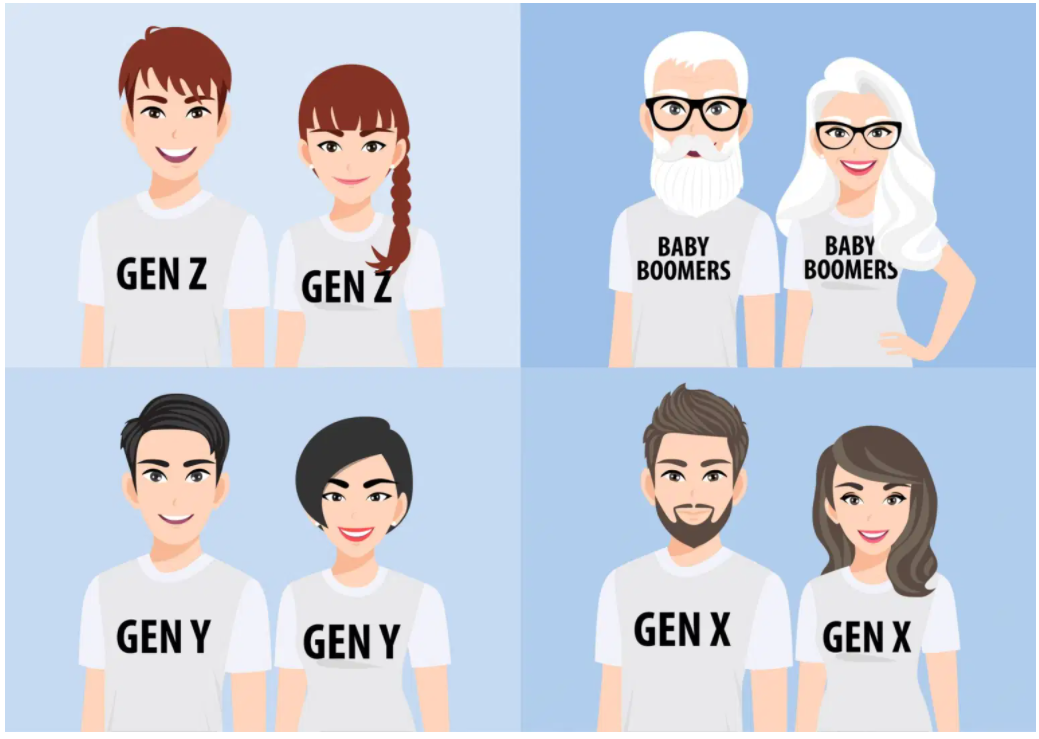
\includegraphics[width=13cm, height=6cm]{"figures/generatii.png"}
			\caption{Generatii}
		\end{figure}
		
		\quad Precum se menționează de relevanță generațiilor la locul de muncă, în cazul nostru se poate discuta despre generațiile de consumator care au evoluat o dată cu tehnologia. Pentru a putea stabili un profil al consumatorului online, ne putem folosi de diferențele dintre generații pentru a analiza decizia de cumpărare a fiecăruia. Astfel, evoluția tehnologiilor informației și comunicațiilor în secolul trecut a dus la dezvoltarea diferitelor etape în evoluția societății. Aceste etape principale de dezvoltare sunt:
		\begin{itemize}
		\item\textbf{Baby Boomers} este generația care e născută între 1946-1964 și care a avut o influență semnificativă asupra schimbărilor demografice din Statele Unite. Economia bine dezvoltată și puternică de după război a oferit oportunitatea și încrederea de a dezvolta familii și de a avea copii. Acest segment este analizat de Kotler, din punctul de vedere al unui consumator, spunând că această generație "\textit{reprezintă reprezintă 76 de milioane de consumatori americani, care posedă 1,2 trilioane de dolari în putere de cheltuieli anuale și controlează trei sferturi din averea țării, comercianții le ignoră adesea}."\footnote{Kotler, Ph., Lane-Keller, K., 2016, Marketing management, 15th Global Edition, Pearson Education, Harlow, England}.
		\item\textbf{Generația X} este născută între 1965-1976. Ei reprezintă prima generație care a început să utilizeze computerul într-un mod similar cu modul în care o facem astăzi. Sunt pricepuți când e vorba de tehnologie, își petrec destul de mult timp pe mediile de socializare, dar sunt încă sceptici când vine vorba de transferuri financiare online.\footnote{Mircea Fuciu, Luigi Dumitrescu, "USAGE OF THE ONLINE BY THE YOUNG ÎNDIVIDUALS AND YOUNG ADULTS. A CASE STUDY OF THE ROMANIAN INTERNET USAGE", 2019, p.41 }
		\item\textbf{Generația Y sau Millennials} este caracterizată prin faptul că s-a născut în 1970-1999/2000.  Sunt cei care apreciază autenticitatea, pun mai mare accent pe ”experiențe”, de la concerte la evenimente sociale, până la preocupări sportive, iar experiența de cumpărare a unui produs cântărește destul de mult în decizia finală.\footnote{Orange, "X, Y, Z sau diferența între generațîi", 13 decembrie 2019, https://www.orange.ro/help/articole/x-y-z-sau-diferența-între-generațîi, accesat în dată de 30.05.2021}
		\item\textbf{Generația Z sau Net Gen} sunt indivizii născuți după 2000. Aproximativ 91\% dintre cei care compun această generație au acces la smartphone și 90\% dintre ei se uită zilnic pe YouTube. Sunt printre primii care au crescut cu social media și tehnologia mobilă – aceasta fiind principala caracteristică generală a acestei generații.\footnote{Ibidem}
		\end{itemize}
		\quad În cadrul acestei lucrări, generațiile de consumatori  care ne interesează pe noi sunt cei din generația Millennials și cei din generația Z deoarece acestea intră în segmentul țintă propus de noi și anume indivizii cu vârstă cuprinsă între 18-30. Consumatorii din Millennials și Net Gen sunt similari în ceea ce privește utilizarea tehnologiei și a internetului, dar aceștia din urmă au un avantaj distinctiv, fiind născuți cu Internetul în viața lor de la o vârstă fragedă. Principalele caracteristici ale celor două generații anterioare sunt mobilitatea și conectivitatea.\footnote{Mircea Fuciu, Luigi Dumitrescu, op.cît, p.42}. În continuare, vor fi prezentate caracteristicile celor două generații pentru a identifica profilul consumatorului din fiecare generație.
	\bigskip
	
		\quad\textbf{ Generația Millennials }\footnote{Imbrea Andra, "Cum vor dicta generațiile Millennials și Z comportamentul de consum în 2020", 2018, www.wall-street.ro, accesat în data de 30.05.2021}
		\begin{itemize}
			\item sunt primii cumpărători online, care au crescut într-un peisaj dominat de giganți online precum Amazon, Alibaba sau eBay, spre deosebire de generația Z care practic s-a născut “cu comerțul electronic”, iar milenarii au pus temelia pentru amploarea pe care a căpătat-o ecommerce-ul.
			\item sunt mult mai dispuși să accepte publicitatea online și mult mai toleranți când vine vorba de servicii și probleme de conectivitate slabă, spre deosebire de generația Z care are zero toleranță când vine vorba de așa ceva.
			\item milenarii preferă să interacționeze cu retailerii sau între ei cu ajutorul canalelor de social media sau aplicațiilor de mesagerie mai degrabă decât vocal sau față în față. Născuți în era cumpărăturilor online, acești consumatori sunt mai înclinați să facă shopping online decât într-un magazin fizic. 
		\end{itemize}
		\quad \textbf{Generația Net Gen}
		\begin{itemize}
			\item a beneficiat de evoluție tehnologică din prima zi și au folosit-o ca pe ceva natural. Astfel, fiind modelați de social media și de tehnologie, ei prețuiesc responsabilitatea socială și impactul pozitiv asupra lumii și sunt interesați de valorile unei afaceri ale căror produse le achiziționează și le pasă mai puțin de pricing decât Millennials.\footnote{Andra Imbrea, op. cît.}
			\item apropierea de tehnologie de la o vârstă mică îi face pe cei din Generaţia Z să aibă o încredere mai mare în tehnologie și mulţi au tendinţa să se numere printre primele persoane care să folosească un gadget sau o tehnologie nouă.\footnote{Loredana Săndulescu, "Generația Z versus Generația Y. Ce îi unește și ce îi diferențiază?", 2020, revistabiz.ro, accesat în dată de 30.05.2021 }
			\item spre deosebire de milenarii, definiți că generația shoppingului online, 67\% dintre tinerii Z preferă să cumpere din magazinele fizice în cea mai mare parte a timpului și 31\% preferă același canal ocazional.\footnote{Andra Imbrea, op. cit.}
		\end{itemize}	
			
		 \quad Pentru a concluziona, putem afirma că aceste două grupuri diferă totuși substanțial în preferințe; dacă Millenialls sunt mai sensibili la prețuri, iar valoarea brandului este mai importantă decât pentru generația Z, aceștia din urmă sunt mult mai atenți la responsabilitatea socială a brandului și mai puțîn toleranți la problemele de conectivitate și la serviciile de calitate inferioară.
	\newpage
		\subsection{Trend-uri in comportamentul consumatorilor online} 
		\quad Un studiu al Comisiei Europene a observat/identificat câteva trend-uri prezente în comportamentul și cererea consumatorilor care au distins numeroasele faciltăți datorate posibilității de a plasa comenzi pe Internet:\footnote{Ibidem, p.21}
		\begin{itemize}
			\item \textbf{Civilizarea și mobilizarea consumului} care implică faptul că e-consumatorii consumă din ce în ce mai mult de acasă sau chiar și când sunt pe drum. În plus, mai există un trend care implică că plasarea de comenzi nu are loc numai unde cumpărătorul dorește dar și la ce ora consideră el. Aceste trenduri sunt facilitate de noi tehnologii precum rețeaua de internet și serviciile de pe telefon la care ai acces 24 de ore pe zi, făcând posibil utilizatorilor să plaseze comenzi oricând au plăcerea și nevoia.
			\item \textbf{Globalizarea} care afectează nu numai producția internațională cât și cererea globală. Consumatorii așteaptă acum produse din toată lumea să fie livrate la ușa casei. Tehnologiile de informare și comunicare au făcut că comerțul dintre diverse țări să fie foarte accesibil iar toți consumatorii din orice parte a lumii să aibă acces la cât mai multe produse similare.
			\item \textbf{Personalizarea}, spre deosebire de producția în masă amintită anterior, drept componentă a globalizării, pune accent pe particularizarea produselor și serviciilor la nevoile individuale ale fiecărui cumpărător astfel încât să aducă un plus valoare acelui bun pentru a crea avantaje competitive.
		\end{itemize}
		\subsection{Factori care influenteaza comportamentul consumatorului online}
	\qquad\space Având în vedere dezvoltarea tehnologiei de-a lungul ultimilor ani,  paradigma achizițiilor a schimbat modul în care cumpărătorii își pot achiziționa diverse bunuri, încurajându-se acum mai mult că niciodată consumul. Astfel, consumatorul contemporan face față la mult mai multe provocări legate de lipsa de timp, multitudinea de opțiuni și volumul de informații disponibile pentru a putea lua o decizie privind procurarea unui produs. Mulți autori au venit cu diferite abordări și studii privind factorii care ar putea influența decizia de cumpărarea a unui e-consumator în zilele noastre.
	
	\quad O abordare foarte interesantă este reprezentată de autorul Paul Henry, care exemplifică constrângerile care afectează comportamentul consumatorului de-a lungul procesului de cumpărare online (figure 1.1).
	\begin{figure}[!htb]
		\centering
		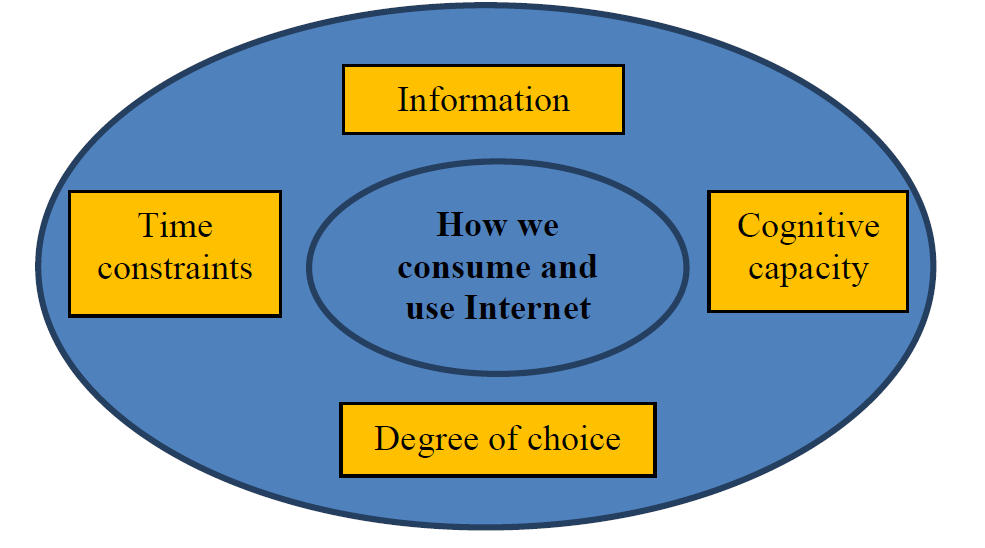
\includegraphics[width=13cm, height=8cm]{"figures/first.png"}
		\caption{Factori de constrângere în procesul de cumpărare al consumatorului}\label{fig:first}
	\end{figure}

	\quad După cum se observă și în figura 1.2 de mai jos, impactul celor patru factori menționați deasupra sunt foarte cunoscuți și relativ ușor de înțeles; Ne aflăm într-o perioada în care cumpărătorul este afectat de presiunea timpului, considerată drept o resursă limitată și rară pe care trebuie să o folosească, să se informeze prin diverse canale media pentru a reuși, în cele din urmă, să facă cele mai bune alegeri dintre opțiunile pe care le oferă piață. Marea provocare rămâne modul în care consumatorul reușește să analizeze, interpreteze și să integreze informația obținută (abilitatea cognitivă) și să o transforme în cunoștințe utile și valoroase.\footnote{Ibidem, p. 23}
	
	\quad  O altă abordare asupra factorilor care influențează achizițiile online ale consumatorilor aparține profesorilor Ujwala Dange and Vinay Kimar(vezi figura 1.3) care au creat modelul "FFF". 
	\begin{figure}[!htb]
		\centering
		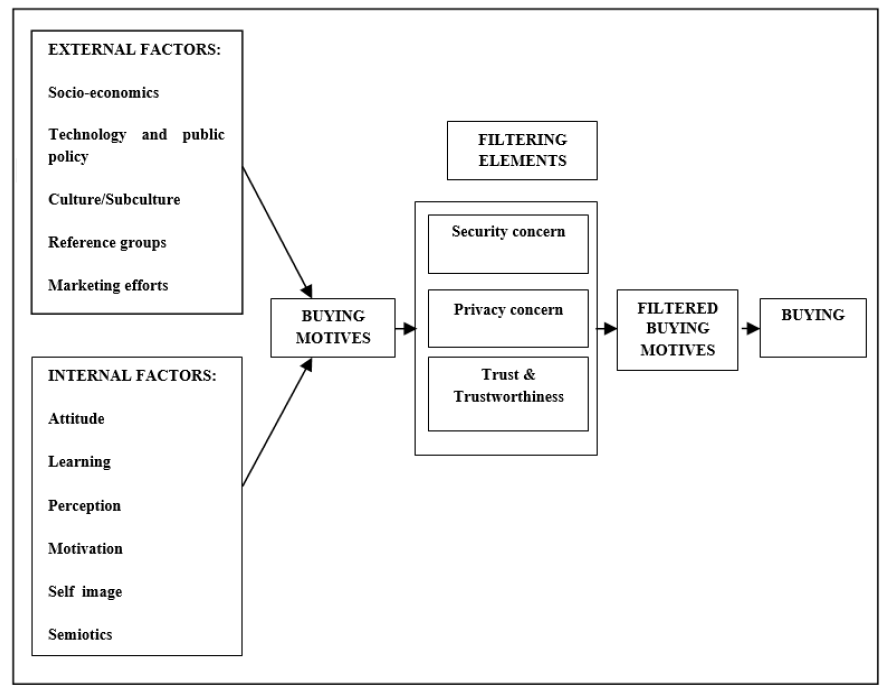
\includegraphics[width=15cm, height=12cm]{"figures/SECOND.png"}
		\caption{Modelul FFF al comportamentului consumatorului online}\label{fig:second}
	\end{figure}
\newpage
	\quad Acest model pornește de la cele trei categorii de influențe exercitate asupra comportamentului cumpărătorului în mediul online și anume: factori interni și externi care pot provoca cumpărătorul să plaseze comenzi online; factorii de filtrare a informațiilor prin prisma riscului perceput de cumpărătorul online și factorii de filtrare a deciziilor de cumpărare, în legătură cu modul în care consumatorul își evaluează propriile așteptări și motive drept un rezultat al acțiunii tuturor influențelor menționate mai sus.\footnote{Ibidem, p.24}
	
	\quad Spre deosebire de abordarea autorului Paul Henry privind impedimentele care ar putea îngreuna procesul de cumpărare și abordarea profesorilor Ujwala Dange și Vinay Kimar, cu modelul celor trei tipuri de factori, se adaugă abordarea lui Ciprian Devderea care, în urmă cercetării perspectivelor pe care alți autori le au asupra factorilor care influențează decizia cumpărătorului de a achiziționa sau nu un produs online, a remarcat trei mari elemente care se evidențiază și care ajută consumatorul să facă alegerea potrivită.\footnote{Ciprian Devderea, "Consumer Behavior Towards Apparel E-Commerce in Romania", p.473-475 }
	\begin{itemize}
		\item\textbf{Calitatea paginii web și anxietatea tehnologică} 
		
		\quad Un element foarte important în comerțul electronic este calitatea web. Pe lângă faptul că are un rol funcțional, calitatea web-ului sau designul site-ului web pot afecta percepția consumatorului și pot influența dacă consumatorul este mulțumit sau nu de ambianță. În plus, accesibilitatea și ușurința folosirii paginii web va determina dacă consumatorul va reveni să mai achiziționeze și alte produse sau va renunța din cauza unor elemente care îi îngreunează plasarea unei comenzi online precum neorganizarea produselor pe categorii, lipsa unor poze reprezentative a bunului achiziționat, solicitarea de prea multe informațîi personale, etc.
		
		\quad Cu toate acestea, dincolo de calitatea experienței online, anxietatea este un subiect frecvent abordat în contextul comportamentului consumatorului online. Anxietatea tehnologică, în contextul cumpărăturilor online, este o reacție negativă care îi influențează pe utilizatori să se îndoiască de capacitatea lor de a efectua o anumită acțiune sau de a-și reduce așteptările cu privire la rezultat.\footnote{Ibidem} Acest lucru înseamnă că utilizatorii au noi griji atunci când achiziționează online, anumite categorii de produse. Un exemplu relevant sunt cumpărăturile online de îmbrăcăminte, în acest caz consumatorii online trebuie să ia în considerare noi elemente precum diferența de dimensiune, diferitele unități de măsurare și alte detalii mici care pot transformă plăcerea cumpărătorilor de a achiziționa într-un stres din cauza incertitudinii.
		
		\item\textbf{Securitatea și confidențialitatea}
		
		\quad Aceste două elemente sunt exprimate prin încrederea pe care consumatorii o au în achiziționare unor bunuri online. Astfel, există diverse studii care confirmă importanța securității și confidențialității informațiilor personale pe care consumatorii trebuie să le ofere în momentul în care plasează o comandă. Din păcate, mulți consumatori evita magazinele online tocmai din cauza acestor doi factori care le generează o atitudine negativă față de mediul digital fie din cauza lipsei de experiență a consumatorului sau a unor experiențe neplăcute din trecut. Însă, în prezent, există reglementări clare și stricte privind drepturile consumatorului online, care au rolul de a oferi utilizatorilor o anumită siguranță.
\newpage
		\item\textbf{Online Word of Mouth} 
		
		\quad Conceptul de Word of Mouth în contextul comerțului electronic(e-WOM) se referă la o conversație online între utilizatori despre un produs sau experiență, care de obicei poate fi negativă sau pozitivă.\footnote{Anastasiei Bogdan, Dospinescu Nicoleta, "Electronic Word-of-Mouth for Online Retailers:
			Predictors of Volume and Valence", 2019, p.2}. Pentru a înțelege mai bine, pot oferi un exemplul tot în contextul cumpărării de îmbrăcăminte online, amintit anterior. În acest caz, se poate lua în considerare actul de interacțiune dintre doi utilizatori care vorbesc despre experiență lor de a comandă un anumit produs de la un anumit magazin online. Astfel, în acest proces, are loc un transfer de informații care vor influență negativ sau pozitiv decizia de a achiziționa din viitor de la acel furnizor online.
		
	\end{itemize}

		\subsection{Procesul de cumparare al consumatorului online}
		\quad\quad După ce am discutat despre lucrurile ce ar putea să determine un consumator să achiziționeze sau nu un produs vom vedea procesul care stă la baza deciziei pe care acesta trebuie să o ia. În primul rând, trebuie să menționăm că în teoria economică tradițională, consumatorul trebuie să acționeze că un individ rațional când vine vorba de achiziția unui bun sau a unui serviciu, punând în balanță costurile și beneficiile ce i se aduc, alegând cea mai bună opțiune care îi satisface complet nevoile.
		
		\quad La baza analizei comportamentului consumatorului online stă procesul decizional al cumpărătorului împărțit pe etapele ilustrate în figura 1.3.\footnote{Eurpean Parliament, \textit{op. cît}, p.38}
		\begin{figure}[!htb]
			\centering
			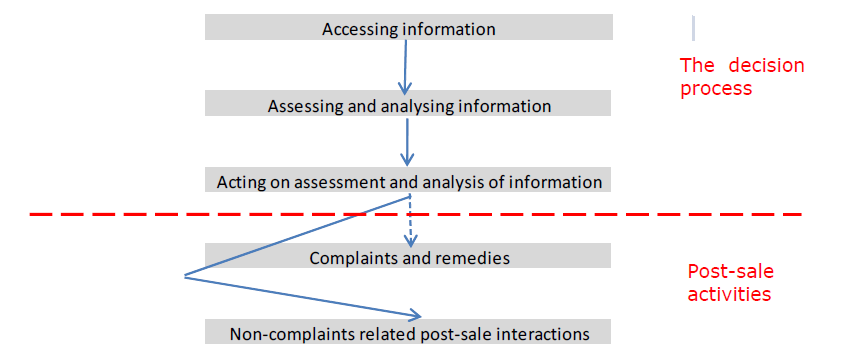
\includegraphics[width=12cm, height=8cm]{"figures/third.png"}
			\caption{Procesul de cumpărare al conumatorului online}\label{fig:third}
		\end{figure}
	
		\subsubsection{Accesarea informației}
		\quad\quad
		 În momentul în care un consumator începe să se gândească la  achiziționarea unui bun, în spatele acestei dorințe stă nevoia pentru un obiect specific sau pentru anumite calități ale acelui produs sau serviciu. Astfel, în această etapă, el începe să consulte toată informația la care poate avea acces pentru a o rezumă și conclude într-o decizie.\footnote{Koetler \& Armstrong, "Principles of Marketing 14th edition, p.153}
		
 		\quad În mediul digital, s-au creat de-a lungul dezvoltării tehnologice diverse motoare de căutare pentru facilitarea găsirii de informații oferind consumatorilor diverse platforme ce comercializează produsele de care e interesat, însă, pe de altă parte, volumul mare de date disponibil online este considerat de unii consumatori drept copleșitor.
		 
	 	\quad De asemenea, consumatorii se bazează  și pe  rețelele de socializare drept un furnizor de informații folositoare pentru decizia lor de cumpărare deoarece acolo regăsesc review-uri și recomandări de la persoane pe care ei le cunosc și le consideră de încredere.\footnote{Orzan Gheorghe, Boboc Larisa- Andreea, Burghelea Ioana, Stupu Diana Luana, "A STUDY OF ONLINE USER’S BEHAVIOUR TOWARDS FACEBOOK SOCIAL NETWORK", 2014, p.3}
		
		\subsubsection{Evaluarea și analiza informației }
		
		\quad\quad După ce consumatorul a adunat toată informația disponibilă online, acesta începe să analizeze opțiunile pe care le are după factorii care reprezintă o importantă pentru el precum brand-ul, calitatea, prețul, reputația produsului etc., și în cele din urmă să aleagă ce tip de produs/ serviciu dorește și de la ce producător să-l achiziționeze. \footnote{Koetler \& Armstrong, \textit{op. cît}}
		
		\quad Neutilizand instrumente de filtrare și sortare a informației, consumatorii tind să ia în considerare doar primele căutări ce le apar în topul listei, uneori bazându-se pe brand-urile pe care ei deja le cunosc în locul celor noi apărute pe piață și netestate înainte fizic.
		
		\quad Cu toate că internetul oferă o multitudine de elemente referitoare la produsele disponibile pe magazinele web, unele produse nu conțîn detaliile semnificative cu privire la componentă lor. Astfel, consumatorii, neavând posibilitatea de a atinge sau miroși produsele înainte de a le cumpără, evita produsele pe care nu le-au încercat în magazinul fizic, deoarece implică o evaluare mult mai dificilă a informației descoperite online.
		
		\quad Se remarcă, de asemenea, faptul că în ciuda volumului mare de informații despre anumite produse sau servicii, sursă de încredere pe care se bazează cel mai mult consumatorii atunci când vine vorba de evaluarea unui produs nou, neincercat, rămân recomandările și părerile persoanelor apropiate sau experiență proprie din trecut.
		
		
		\subsubsection{Luarea deciziei}
		
		\quad\quad În această etapă consumatorul a înțeles nevoia care trebuie să fie satisfăcută, a parcurs toate și analizat informațiile necesare luării unei decizii și urmează să-și plaseze comandă online de la producătorul care reușește să îndeplinească toate criteriile care prezintă relevanță și importantă pentru cumpărător.
		
		\quad  Comerțul electronic îi oferă cumpărătorului diverse avantaje precum o varietate largă de produse, posibilitatea de a plăti un preț mai mic pe un produs ce se regăsește și în magazinul fizic, dar și unele riscuri precum utilizarea datelor personale pentru alte scopuri  fără consimțământul lor și frică de costurile extra, ascunse, strategie folosită de unele firme și cunoscută drept "drip-pricing".\footnote{European Parliament, \textit{op.cît} p.52}
		
		\subsubsection{Mecanismul de reclamații și recurs}
		
		\quad\quad Este necesar de menționat că această etapă se aplică numai atunci când consumatorul are o problema cu produsul sau serviciul livrat și vrea să facă o reclamație către producător. Procesul de cumpărare într-o piață digitală diferă de procesul consumatorului offline care achiziționează din magazinul fizic, unde are posibilitatea de a observă și analiză toate calitățile și defectele unui anumit bun. Prin urmare, atunci când cumpărătorii achizitioneza în mediul online e posibil că ei să experimenteze o schimbare în tipul și magnitudinea problemei pe care o întâlnesc față de cele în magazinele fizice, implicând de asemenea riscuri mai mari.
		
		\quad Se consideră că un consumator rațional s-ar plânge către vânzător dacă întâmpină o problema cu produsul sau serviciul livrat însă, în realitate nu toți cumpărătorii aleg să revină cu un feedback și să facă o sesizare despre defectele surprise, din diverse motive personale, iar acest lucru este și mai dificil într-un mediul online spre deosebire de cel fizic.\footnote{Ibidem, p.90}
		
		\quad În mare parte din problemele pe care un consumator le poate experimenta în momentul în care plasează o comandă online au legătură cu  modul de livrarea și cu calitatea promisă pe care descrierea de pe site sugerează că o deține un anumit produs și care în momentul primirii coletului se denotă contrariul așteptărilor.
		
		\subsubsection{Serviciile și interacțiunile post-vanzare}
		
		\quad\quad Unii producători apelează la interacțiunile și serviciile post-vânzare între cumpărător și firma pentru a crea o legătură de lungă durata care îl va determina pe consumator să mai plaseze și alte comenzi în viitorul apropiat.\footnote{Ibidem, p.98} Aceste strategii de promovare, constă în comunicarea de promoții la pachete de produse, reduceri disponibile pe site-ul web, vouchere periodice pentru fidelizarea clienților etc. Cu toate că aceste oferte ar putea sună atractive la prima vedere, unii consumatori consideră că trimiterea unor astfel de email-uri, fără permisiunea lor, poate fi considerată drept o inițiativa time consuming și care creează iritare.
		
		\subsection{Beneficiile si provocarile achizitiilor online}
		
		\quad De-a lungul experiențelor consumatorilor, privind achizițiile în mediul online, s-au remarcat diverse avantaje care i-a determinat pe consumatori să pășească în piață digitală pentru a-și satisface nevoile sau dorințele personale. Printre acestea enumerăm: 
		\begin{itemize}
			\renewcommand{\labelitemi}{$\Rightarrow$}
			\item Oportunitatea de a plăti prețuri mai mici deoarece în mediul digital magazinele online plătesc costuri mai mici față de magazinele fizice, de exemplu chiria.
			\item  Accesul la o varietate mai mare de produse și producători. Acest lucru reprezintă o importantă mare pentru zonele sărace în care nu sunt atât de dezvoltate magazinele clasice.
			\item Posibilitatea de a achiziționa un bun la orice ora și oriunde dorește consumatorul în limita stocului disponibil de pe site.
			\item Creșterea ușurinței comparației caracteristicilor produselor cu ajutorul anumitor platforme sau chiar compararea aceluiași produs dar de la diferiți producători.
			\item Abilitatea de a  oferi și de a primi recomandări și păreri care pot ajută consumatorii să ia o decizie asupra procesului de cumpărare al unui anumit bun.
		\end{itemize}
		
		\quad Cu toate că dezvoltarea piețelor de desfacere a dus la extinderea lor și în mediul digital iar majoritatea consumatorilor au început să fie atrași mai mult de beneficiile cumpărării de pe platforme online, unii cumpărători au întâmpinat și probleme care i-a determinat să se gândească de două ori atunci când doresc să plaseze o comandă online. Printre aceste probleme s-au remarcat: 
		\begin{itemize}
			\renewcommand{\labelitemi}{$\Rightarrow$}
			\item Non-livrarea sau întârzierea livrării unui produs care menționa că ajunge într-un anumit interval de timp și a depășit cu mult timpul de așteptare. 
			\item Bunurile care nu s-au prezentat la momentul livrării conform caracteristicilor afișate pe site-ul producătorului.
			\item Diverse probleme referitoare la garanția unor produse cum ar fi în cazul electronicelor care au garanție pe o perioada mai mare de timp.
			\item  Bunuri care la momentul deschiderii ambalajului aveau defecte iar producătorul nu avea o politică de return privind produsele cu probleme.
			\item Riscurile privind securitatea și protecția datelor personale furnizate necesare livarii la domiciliul consumatorului a produsului sau serviciului.
			\item Costurile sau prețurile care nu sunt afișate complet pe anumite site-uri ale producătorilor.
		\end{itemize}
\newpage
	\subsection{Asemanari și deosebiri între e-commerce și comerțul fizic}
	\begin{figure}[!htb]
		\centering
		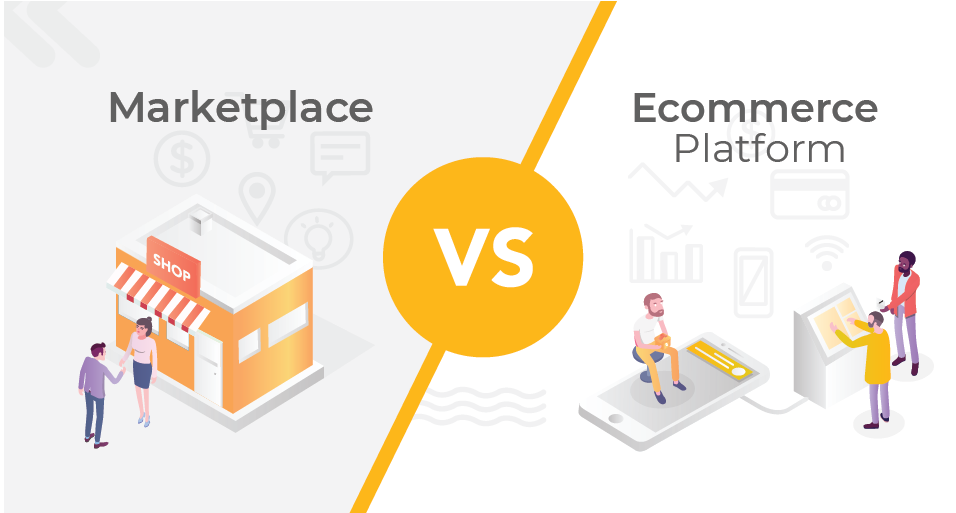
\includegraphics[width=13cm, height=6cm]{"figures/magazin.png"}
		\caption{Magazine fizice vs Magazine online}
	\end{figure}
	
	\quad Se poate afirmă că există diverse opinii și articole referitoare la asemănările și deosebirile dintre mediul online și offline privind cumpărăturile consumatorilor, spunând că mediul digital și procesul de cumpărare online este total diferit de cel fizic datorită anumitor elemente sau bariere care facilitează sau îngreunează achiziția de bunuri și servicii. În următoarele rânduri vor fi prezentate câteva dintre argumentele care subliniază diferențele dintre cele două modalități prin care un cumpărător poate achiziționa un produs și apoi cele care evidențiază asemănările dintre cele două.
	\bigskip
	
	\quad \textbf{Diferențe}
	\begin{itemize}
		\item Mediul online este foarte diferit  de mediul fizic din cauza imposibilității reacțiilor senzoriale asupra unui produs pentru a testa veridicitatea calității produsului.\footnote{Anca-Maria Milovan-Ciuta, "PERSONALITY INFLUENCES ON ONLINE STORES CUSTOMERS BEHAVIOR", 2015, p. 70-71} Astfel, consumatorii online nu au oportunitatea de a valida informațiile prezentate pe site-ul magazinului, bazându-se doar pe review-urile celor care au achiziționat anterior produsul. În magazinele fizice, consumatorii au oportunitatea de a atinge produsul înainte de cumpărare, verificând caracteristicile pe loc.
		\item Mediul online nu oferă posibilitatea primirii produsului într-un timp cât mai scurt, deoarece un proces de ambalare, pregătire și livrare durează, în medie, 1-2 zile. În acest caz, nu putem vorbi de caracterul urgent, care nu este posibil în magazinele digitale. În magazinele fizice, caracterul urgent poate fi facilitat de magazinele care sunt deschise în limita stocului disponibil și a programului fiecăruia.
		\item Mediul online nu oferă posibilitatea de interacțiune între comerciant și consumator, deoarece consumatorul folosește o platforma prin care își selectează și plasează comenzile cu produsele dorite, iar în caz de erori ale produsului, politică de return poate să fie mult mai complicată, implicând mai mulți pași.\footnote{Ibidem} În magazinele fizice, există o clară interacțiune între vânzător și cumpărător, care poate facilita uneori procesul decizional de cumpărare, iar politică de return se rezumă la întoarcerea produsului în stare bună în magazinul de unde a fost achiziționat, fără a fi nevoie de alți pași sau costuri suplimentare.
	\end{itemize}
	\quad \textbf{Asemănări}
	\begin{itemize}
		\item Ambele tipuri de magazine deservesc același scop, acela de a satisface nevoile consumatorului prin oferirea unei game de produse din care consumatorul poate alege liber și necondiționat de nimeni.
		\item În ambele cazuri are loc derularea unui proces decizional de cumpărare în urmă căruia consumatorul analizează informațiile disponibile, fie ele din surse online sau de la persoane apropiate și decide să achiziționeze produsul potrivit acestuia. 
		\item Ambele necesită acțiuni de promovare a produselor pe care le comercializează. Indiferent că sunt magazine online sau fizice, acestea trebuie să se evidențieze pe piață și să-și crească vizibilitatea în față consumatorilor pentru a-i atrage cu produsele proprii.
	\end{itemize}
	
	\newpage
	\section{Cercetare secundara privind comportamentul consumatorului online, roman, tanar si educat}
	
	\quad\quad Comertul electronic in Romania este o piata in continua dezvoltare ce duce la aparitia unui comportament nou de cumparare. In acest capitol se analizeaza situatia din Romania privind numarul de achizitii online ale consumatorilor romani si factorii care influenteaza cumparaturile online. In a doua parte se prezinta, pe scurt, trei articole care constituie cercetarea secundara si care au analizat comportamentul consumatorului online, tanar si educat din Romania.
	
	\subsection{Comertul electronic in Romania}
	\qquad  În România, piața de comerț electronic și-a făcut prezența la inceputul anului 2004\footnote{Obrad Ciprian, Vasile Gherghes, "ATTITUDES TOWARDS ONLINE COMMERCE: A CASE STUDY OF STUDENT POPULATION IN TIMIȘOARA", 2016, p.47} și a început să se dezvolte cu adevărat cu admiterea țării în Uniunea Europeană atunci când fondurile europene pentru investițiile în infrastructură au început să fie accesibile. Chiar dacă acest lucru a fost un beneficiu pentru dezvoltarea comerțului electronic în România și în prezent conform statisticilor naționale, 55,8\% din gospodăriile din România au un computer la domiciliu (INS 2013) și 54,4\% din gospodării atât în zonele rurale, cât și în cele urbane au acces la Internet, rata cumpărăturilor online rămâne destul de scăzută în Europa de Est, inclusiv în România (INS 2014). In cele din urma, decizia de a cumpăra online este, de asemenea, influențată si de factorii culturali.\footnote{Onete, C. B., Teodorescu, I. and Vasile, V., 2016. "Considerations Regarding the Analysis of the Digital Consumer in Romania. Amfiteatru Economic", p. 656}
	
	\qquad Comerțul electronic a devenit din ce în ce mai prezent pe lista românilor de opțiuni de cumpărături, în contextul unei rate de penetrare a internetului în creștere: "Deși penetrarea pe Internet în România este încă scăzută în comparație cu media europeană de 70\%, până în 2018, ratele sunt asteptate să fie semnificativ mai echilibrate cu peste două treimi din populația care are acces la domiciliu la Internet "(Euromonitor, 2014).\footnote{Claudia Bobalca, \textit{op.cit}, p.241}
	
	\quad Privind contextul achizitiilor online, românii cumpără în cea mai mare parte electronice și jocuri video, îmbrăcăminte, produse de frumusete si produse de ingrijire personala. Cu tot mai mulți clienți care trec la cumpărăturile online și o rată în continuă creștere a prezenței online a comercianților cu amănuntul pe piața românească, o mare provocare pentru manageri, este de a atrage noi clienți, formând  totodata și clienți loiali.\footnote{Ibidem, p.242} Cu cat exista mai mult acces la informații și având deja o experiență de cumpărare, obiceiurile de cumpărături online ale românilor sunt în continua dezvoltare. Noua generație de tineri este mai familiarizată cu tehnologia online, are mai multă experiență în utilizarea internetului și este mai dispusa să se confrunte cu riscurile percepute de achizitiile online.
	
	\quad Un alt factor important care a favorizat achizitiile online in ultima perioada este pandemia Covid19 care a afectat intreaga lume, inclusiv Romania.\footnote{Claudia Gorunescu, Ecommerce in timpul convid-19: Ce impact resimte piata din Romania, accesat in data de: 25.04.2021}. Astfel, multi antreprenori romani s-au mutat in mediul online pentru a-si putea salva afacerile din cauza restrictiilor impuse pentru protejarea cetatenilor si a consumatorilor.Exista date statistice care sublinieaza o crestere a cumparaturilor online in randul romanilor in aceasta perioada precum figura 2.1 de mai jos care arata o comparatie intre frecventa cumpararaturilor online inainte, in timpul si dupa pandemia Covid19.\footnote{Statista 2021,https://www.statista.com/statistics/1169383/romania-online-shopping-frequency/, accesat in data de 15.04.2021.} dar si articole care subliniaza aceasta crestere("În timpul pandemiei Covid-19, consumatorii români au avut tendința de a cumpăra mai multe produse locale, în special mărfuri de bază.")\footnote{Nistor Andra,COVID-19 Transforms Romanian Retail and Food Service Sectors, 2020, p.3}
	 	\begin{figure}[!htb]
	 	\centering
	 	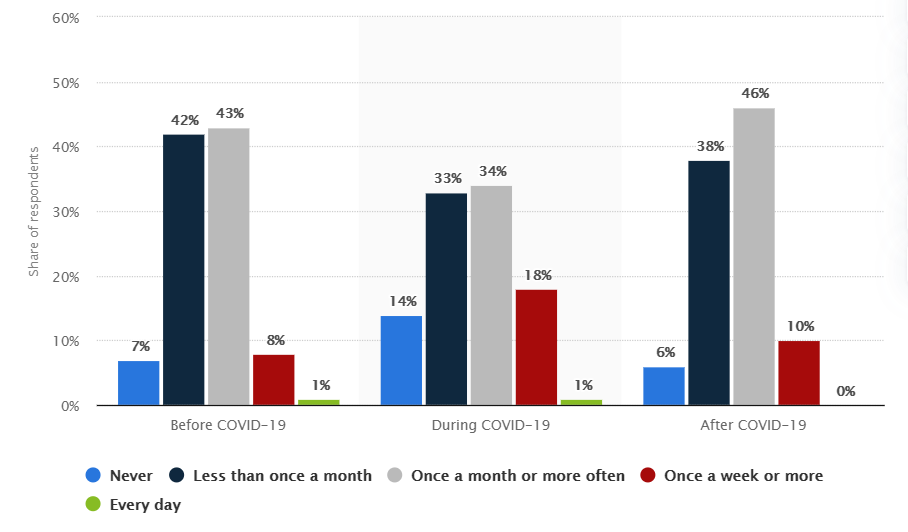
\includegraphics[width=11cm, height=6cm]{"figures/fourth.png"}
	 	\caption{ Frecventa cumparaturilor online in Romania 2020-2021}\label{fig:fourth}
		 \end{figure}
\newpage 
 \qquad Pentru a aduce informatii noi privind comportamentul consumatorilor online tineri si educati din Romania a fost necesar parcurgerea a mai multor articole care furnizau date despre ecommerce-ul din Romania. In cele din urma, trei articole s-au evidentiat deoarece detineau drept subiect comportamentul consumatorului online si tanar din Romania cu varste cuprinse intre 18-35 de ani. Am impartit cele trei articole in trei studii caz A, B si C pe care le voi face prezenta pe scurt prin prisma elementelor prin care se diferentiaza si prin informatiile noi aduse despre comportamentul consumatorului online tanar si educat din Romania.
 \subsection{Cercetarea A}
 Studiul de caz "A" este scris in 2016 si publicat in Amfiteatrul Economic  de trei autori: Cristian Bogan Onete, Ioana Teodorescu si Viorel Vasile; Articolul surprinde o analiza asupra componentelor comportamentului consumatorului digital din Romania in contextul evolutiei cumparaturilor online. Studiul incepe cu informatii generale despre nivelul comertul electronic la nivel de Uniune Europeana, la nivel de tara si aduce un plus de valoare cu  factori predominanti care influenteaza alegerea unui consumator roman inainte de a achizitiona online afisati in tabelul din figura 2.2.\footnote{Onete, C. B., Teodorescu, I. and Vasile, \textit{op.cit}}
 	\begin{figure}[!htb]
 	\centering
 	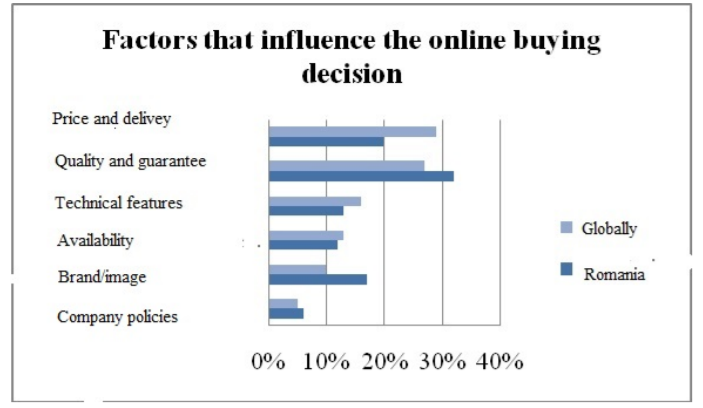
\includegraphics[width=12cm, height=8cm]{"figures/fifth.png"}
 	\caption{Factori care influenteaza decizia de cumparare online a romanilor}\label{fig:fifth}
 \end{figure}

		\quad  Potrivit acestui tabel am descoperit că consumatorii digitali români sunt influențați cel mai mult de calitatea și garantarea unui produs / serviciu (32\% în România, 27\% la nivel global). În România, cel mai important factor pare a fi calitatea și garanția unui produs, în timp ce respondenții la nivel global sunt influențați cel mai mult prin preț și livrare (29\%), după cum se poate observa în figura 5. Termenii de preț și de livrare se situează pe locul doi în opinia respondenților români (20\% în România, 29\% la nivel global), în timp ce marca / imaginea este, de asemenea, un factor decisiv pe care consumatorii îl iau în considerare (17\% în România, 10\% la nivel global ).
		
		\quad Scopul principal al lucrării este de a înțelege comportamentul românesc digital al consumatorilor incepand cu motivul pentru care românii preferă să cumpere produse / servicii pe piețele externe pe Internet si pana la identificarea factorilor care influenteaza comportamentul consumatorului. Metoda de preluare a datelor a fost un chestionar electronic administrat la 160 de utilizatori de social media, din mediul urban, educati, cu varste cuprinse intre 20-35 de ani.
		
		\quad Conform rezultatelor, chestionarul a fost completat 74\% de femei si 26\% de barbati. Printre intrebarile sondajului, s-a evidentiat intrebarea 3 care arata pietele principale comerciale online de la care romanii achizitioneaza online, afisate in figura 2.3. 
		\begin{figure}[!htb]
			\centering
			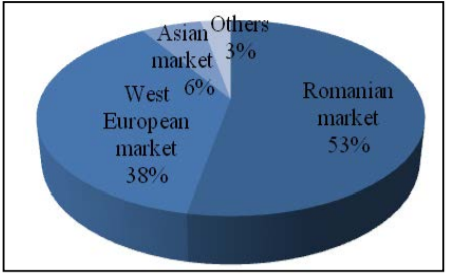
\includegraphics[width=10cm, height=6cm]{"figures/sixth.png"}
			\caption{Online markets}\label{fig:sixth}
		\end{figure}
	
	\qquad O alta intrebare relevanta comportamentului consumatorului online din Romania a fost motivele pentru care romanii cumpara de la producatori din afara tarii, reprezentate in figura 2.4.
	\begin{figure}[!htb]
		\centering
		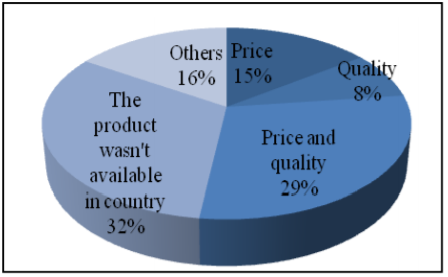
\includegraphics[width=10cm, height=6cm]{"figures/seventh.png"}
		\caption{Motive pentru a cumpara de la producatori straini}\label{fig:seventh}
	\end{figure}
\newpage
	\quad Ultima intrebare relevanta arata categoriile de produse pe care consumatorii online din Romania le cumpara de la producatorii din strainatate in mod frecvent, afisate de asemenea, prin figura 2.5 reprezentativa a rezultatelor. Acest lucru denota faptul ca românii își satisfac nevoile existențiale într-o manieră mai convenabilă, economisind timp fără a fi nevoie să caute produse într-un magazin tradițional.
		\begin{figure}[!htb]
			\centering
			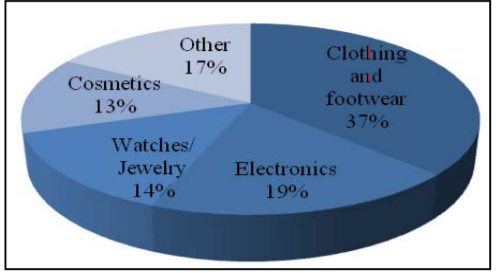
\includegraphics[width=10cm, height=7cm]{"figures/eigth.png"}
			\caption{Categorii de produse cumparate din strainatate}\label{fig:eigth}
		\end{figure}
	
		
	\subsection {Cercetarea B}
	\qquad Studiul de caz B este scris in 2013 si publicat in "Procedia Economics and Finance" de trei autori: Georgiana Bighiu, Adriana Manolica*, Cristina Teodora Roman. Prin aceasta lucrare se doreste a se afla daca CBD ( tulburarea de cumparare compulsiva ) se regaseste in randul studentilor din Romania care cumpara online. CBD este definita in articol drept acel „tip de comportament al consumatorului care este inadecvat, de obicei excesiv și clar perturbator pentru viața indivizilor care par impulsivi să consume”.\footnote{Bighiu Georgiana, Manolica Adriana, Roman Teodora Cristina, "Compulsive buying behavior on the internet", 2015, www.sciencedirect.com} In continuarea articolului  este specificata si explicata clar diferenta dintre achiziitle compulsive si impulsive: cumpararea compulsiva fiind atunci cand dorinta de cumparare vine din interior, poate chiar o anxietate interioara care se calmeaza prin procesul de cumparare pe cand cumpararea impulsiva este determinata de factori exteriori.
	
	\quad Studiul vizează identificarea  populației de studenți români care suferă într-un anumit grad de CBD în comportamentul lor de cumpărături online și care sunt factorii care îl favorizează. De asemenea, se sustine ideea ca stiind ce îi determină pe consumatori să cumpere fără să aibă un procesul decizional prelungit este util în proiectarea promoțiilor pentru site-urile online care vând, de exemplu, cupoanele.  
	
	\quad Obiectivul principal al studiului este de a analiza comportamentul cumpărăturilor online și de a construi un profil al studentului român ca cumpărător online compulsiv / non-compulsiv.
	
	\quad Metoda de culegere a datelor in cazul acestui studiu este tot chestionarul. Autorii au "imprumutat" adaptat si tradus in romana un chestionar de la o cercetare in italiana privind acelasi subiect. La sfarsitul colectarii de informatii s-au obtinut 100 chestionare valide de la studentii facultatii De Economie si Administrarea Afacerilor. 
	
	\qquad In urma rezultatelor obtinute s-au remarcat urmatoarele informatii: 
		\begin{itemize}
	\item dintre respondenti 81\% erau studenti de la licenta iar 19\% de la master. 
	\item Studentul FEAA folosește internetul de aproximativ 8 ani, iar in ceea ce privește obiceiurile sale de cumpărare online, cumpără online 2 produse pe lună și 19 produse pe an, în medie. In ciuda dezvoltarii metodelor de plata, studentii prefera plata traditionala in cash a produselor/serviciilor achizitionate.
	 \item În ceea ce privește articolele cele mai achiziționate online, cele mai des alese au fost articolele de îmbrăcăminte (alese de 57 de respondenți), rezultat care poate fi explicat prin faptul că două treimi dintre respondenți au fost femei, electronice sau articole de uz casnic (60/100) , bilete (autobuz, tren, avion; 49/100)
	\item Un procent de 13\% dintre respondenți s-a dovedit a avea un scor în concordanță cu tulburarea de cumpărare compulsivă. Dintre aceștia, 84,6\% erau femei, iar restul de 15,4\% bărbați confirmând rezultatele cercetării Guerreschi (2012) că majoritatea cumpărătorilor compulsivi sunt femei.
\end{itemize}
		\qquad In concluzie, profilul consumatorului compulsiv online este similar cu cel găsit în literatura scrisă despre această dependență și care confirmă studiile anterioare. Shopaholic este femeia (84,6\% dintre studenții cu CBD) cu o vârstă medie de 20 de ani, când apar de obicei primele semne ale patologiei.
		
		\quad Pe de altă parte, studentul „obișnuit” este încă blocat în modul tradițional de cumpărare demonstrând neîncredere în metodele de plată online. El / ea preferă plata la livrare care, cumva,  reduce riscul de cumpărare compulsivă, deoarece comanda poate fi anulată spre deosebire de plățile cu cardul dacă ar fi mai mult dificil. Cu toate acestea, el / ea cumpără online 19 produse pe an, indiferent dacă este vorba de haine, electronice sau bilete etc.
		\subsection{Cercetarea C}
		\qquad Ultimul studiu de caz  a fost scris tot in 2013 si publicat in revista CES Working Papers de catre Claudia Bobalca.Scopul cercetării este de a investiga percepția clienților online români cu privire la procesul de cumpărare a produselor de pe Internet. Articolul incepe cu definirea comertului electronic drept orice forma de tranzactie comerciala unde partile interactioneaza intr-o maniera electronica.\footnote{Claudia Bobalca, \textit{op.cit}, p.241}
		
		\quad Obiectivele cercetarii sunt de a afla: avantajele si dezavantajele cumparaturilor de pe internet, motivele pentru care romanii cumpara de pe Internet si motivele pentru care aleg sa cumpere de pe acelasi site.
		
		\quad In acest caz, metoda de culegere a datelor a fost interviul semi-structurat. Populatia investigata este reprezentata de clientii online din Romania care obisnuiesc sa cumpere produse de pe un site specific. 
		
		\quad Eșantionul final a fost compus din 20 de bărbați și 10 femei, deoarece cercetările de afaceri arată o rată mai mare de bărbați cumpărători online din România. Principalele produse cumpărate de participanți din magazinele online sunt: îmbrăcăminte (26 de răspunsuri), produse electronice (23 de răspunsuri), încălțăminte (17 răspunsuri), produse cosmetice (10 răspunsuri) și accesorii (7 răspunsuri).
		
		\quad Primul obiectiv a fost identificarea avantajelor și dezavantajelor cumpărăturilor online. 
		 
		 \quad Lucrarea a reprezentat prin doua figuri. In tabelul cu beneficiile achizitiilor online este scris frecventa avantajelor pe care le-au ales respondentii in urma raspunsurilor date. Astfel, figura 2.6 este o organizare a acestor elemente favorabile mediului online organizate pe 5 dimensiuni.
		\begin{figure}[!htb]
			\centering
			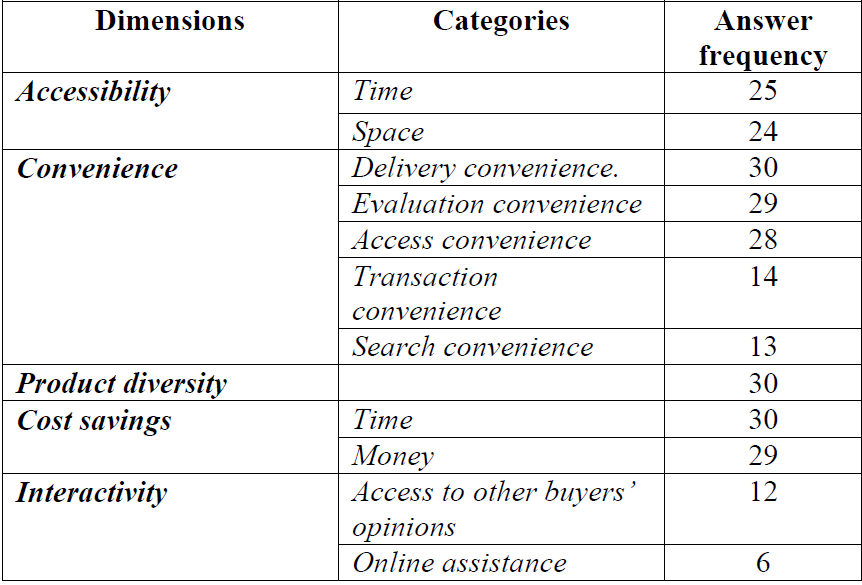
\includegraphics[width=11cm, height=8cm]{"figures/zece.png"}
			\caption{Avantajele achizitiilor online}\label{fig:zece}
		\end{figure}
	
	\begin{enumerate}[a.]
		
\newpage		
	\item\textbf {Accesibilitatea} este reflectată de două categorii: timp și spațiu. Cumpărarea de pe Internet elimină restricțiile de timp. De asemenea, nu există restricții de spațiu deoarece produsele pot fi cumpărate la orice oră din orice țară.
	\item\textbf{Convenienta} este formata din 5 categorii: 

	\begin{itemize}
		\item\textbf{ Acces comoditate.} Majoritatea respondenților consideră că a cumpăra de pe Internet înseamnă că nu mai trebuie să mergi într-un magazin,iar astfel poți evita locurile aglomerate.
		\item\textbf{Comoditate de căutare.} O treime dintre respondenți consideră că Internetul oferă posibilități mai bune de căutare a produselor decât magazinele tradiționale.
		\item\textbf{Confortul evaluării.} Aproape toți respondenții consideră că cumpărarea online facilitează o selecție foarte bună a produselor și produse și / sau prețuri mai eficiente și detaliate comparații. De asemenea, confortul evaluării include mai mult timp pentru respondenți să gândească, să evalueze.
		\item\textbf{Comoditatea tranzacției.} Aproximativ jumătate dintre respondenți consideră că un alt avantaj este comoditatea tranzacției: de asemenea, apreciază posibilitățile de plată.	
		\item\textbf{Confort de livrare.} Toți respondenții consideră că livrarea la domiciliu este foarte importantă si menționează si posibilitatea de a returna un produs.
	\end{itemize}
		\item\textbf{Diversitatea produselor} Toți respondenții apreciază că magazinele online oferă o mare diversitate de produse, mult mai mare uneori decât magazinele tradiționale.
		\item\textbf{Reducerea costurilor} este formata două categorii pentru dimensiunea de economisire a costurilor
	\begin{itemize}
		\item\textbf{Economisire de timp.} Toți respondenții consideră acest avantaj important.
		\item\textbf{Economie de bani.} Aproape toți respondenții menționează prețuri mai bune pentru produsele online, multe oferte speciale disponibile în mediul online și costul de livrare gratuit sau mic.
	\end{itemize}
	\item\textbf{Interactivitate} cuprinde doua categorii:
	\begin{itemize}
		\item\textbf {Acces la opiniile altor cumpărători.} Unii respondenti au spus că cumpărarea online permite clienților să acceseze feedback-ul de la alte persoane care au cumpărat de pe același site web sau din aceleași produse
		\item\textbf{Asistență online.} Unii respondenți consideră că asistența online este un avantaj.
	\end{itemize}
	\quad In continuare sunt reprezentate dezavantajele care au rezultat din raspunsurile date de respondenti. Acestea sunt organizate in figura 2.7 si impartite, pentru a fi intelese mai usor, in cinci dimensiuni.
	\end{enumerate}
		\begin{figure}[!htb]
		\centering
		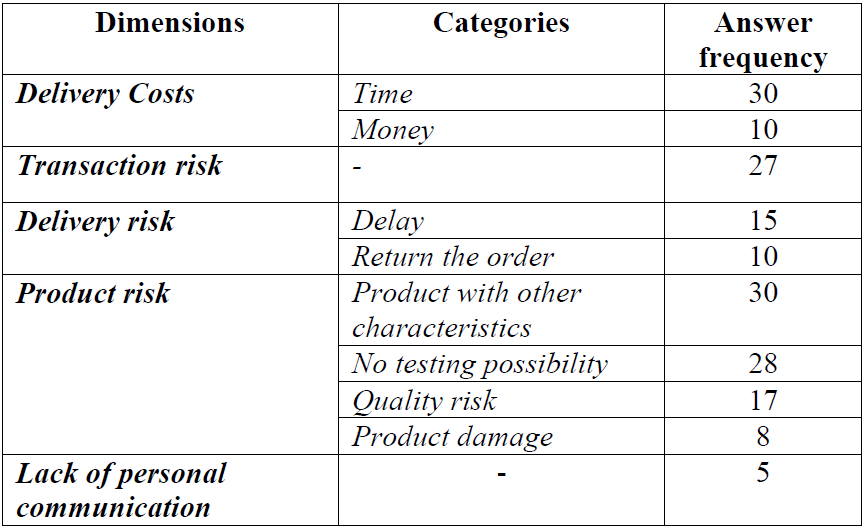
\includegraphics[width=11cm, height=8cm]{"figures/noua.png"}
		\caption{Dezavantajele achizitiilor online}\label{fig:zece}
	\end{figure}
	\begin{enumerate}[a.]
		\item \textbf {Costurile de livrare} se impart in 2 categorii:
	\begin{itemize}
		\item\textbf{Banii} O treime dintre respondenți consideră că plata costului de livrare este un inconvenient și că toate site-urile web ar trebui să aibă taxe de livrare gratuite.
		\item\textbf{Timp.} Toți respondenții au fost de acord că a cumpăra de pe Internet înseamnă a nu primi produsul pe care l-ați cumpărat la timp în aceeași zi.
	\end{itemize}
	\item\textbf{Riscul tranzacției.} În ceea ce privește riscul tranzacției, 27 de respondenți consideră că metodele de plată nesigure reprezintă o mare problemă în România.
	\item\textbf {Riscul de livrare}
		Jumătate dintre respondenți menționează ca posibile dezavantaje în ceea ce privește livrarea faptul că produsele pot îmbogăți destinația cu mare întârziere.
	\item\textbf{Riscuri privind produsele} se impart in 4 categorii:
	\begin{itemize}
	\item \textbf{Daune ale produselor.} Câțiva respondenți menționează ca dezavantaj riscul ca produsul să fie deteriorat în timpul livrării.
	\item\textbf{Produs cu alte caracteristici.} Riscul ca produsul să nu fie același cu cel comandat de un cumpărător este o mare problemă pentru toți participanții.
	\item\textbf{Risc de calitate.} Mai mult de jumătate dintre respondenți consideră că riscul de calitate este o problema importanta în comerțul electronic.
	\item\textbf{Nicio posibilitate de testare.} Faptul că produsele nu pot fi văzute, atinse sau testate înainte de cumpărături este, de asemenea, un dezavantaj menționat de participanți.
	\end{itemize}
	\item\textbf{Lipsa comunicării personale.}
		Cumpărăturile online se caracterizează printr-o lipsă puternică de comunicare personală.
		
		\quad In cadrul ultimelor doua obiective au reiesit ca cele mai importante motive pentru care participanții folosesc pentru a cumpăra din magazinele online sunt: accesibilitatea spațiului, comoditatea accesului, confortul evaluării, comoditatea livrării, economisirea timpului și economisirea banilor; iar motivațiile pentru repetarea achiziției de pe același site web sunt: calitatea produselor, diversitatea produselor, livrare rapidă, ușor de utilizat, recomandări, oferte bune, siguranță, reputație și interactivitate.
	\end{enumerate}
\bigskip
		\quad Aceste cercetari au avut fiecare o perspectiva unica deoarece cercetarea A, fiind un articol mai recent (2016) se focuseaza pe evolutia cumparaturilor online avand in vedere perspectiva consumatorilor online din Romania asupra extinderii comertului electronic inafara granitelor din 2018; Cercetarea B, are de asemenea o abordare unica asupra unui concept aplicat in contextul achizitiilor online si anume CBD (tulburarea de cumparare compulsiva) dorind sa afle daca acest comportament se intalneste si al consumatorii online;iar Cercetarea C se concentreaza pe analiza avantajelor si dezavantajelor pe care consumatorii online, tineri si educati din Romania le-au intalnit de-a lungul experientelor lor.
		 
		\quad Astfel, daca am contopi toate informatiile importante de la fiecare studiu de caz, am putea spune ca avantajele si dezavantajele detaliate in cercetarea C se regasesc si in cercetarea A chiar daca exista o diferenta de 3 ani intre articole, fapt ce demonstreaza ca principalele motive pentru care consumatorii online din Romania achizitioneaza in mediul digital s-au pastrat. De asemenea, am regasit si o contradictie intre cercetarea B si cercetarea C cu privire la genul care achizitioneaza cel mai mult online si anume prima cercetare afirmand femeia cumpara cel mai des, iar a doua cercetare spunand ca barbatii.
	
	
	
\newpage	
	\section{Studiu de caz }
	
	\quad\quad  Prin acest capitol se urmareste realizarea unui profil al consumatorului online, tanar si educat din Romania pentru ca firmele ce utilizeaza comertul electronic sa inteleaga mai bine comportamentul acestuia si sa se plieze pe nevoile si dorintele lui. De asemenea, acest capitol reprezinta partea practica a prezentei lucrari de licenta si are rolul de a identifica elementele care creaza profilul consumatorului online, tanar si educat din Romania. Datele colectate si rezultatele obtinute in urma prelucrarii si interpretarii constituie o baza pentru organizatiile care doresc sa-si constituie strategii de marketing orientate spre consumator.
	\subsection{Scop si obiective}
	\qquad In ultimii zece ani, afacerile din Romania s-au extins din ce in ce mai mult o data cu dezvoltarea mediului online, oferind o gama mult mai larga de produse, fapt ce a oferit posibilitatea oricarui consumator de a cumpara oricand si oriunde s-ar afla, doar printr-o simpla conectare la internet. Astfel, magazinele online au devenit foarte accesibile pentru populatia tanara si educata din Romania, nascuta dupa anii `90 si care este obisnuita cu boom-ul tehnologic. Aceasta cercetare isi propune sa realizeze profilul  acestui consumator online, tanar si educat din Romania.  Aceasta informatie poate fi de folos  firmelor prezente in mediul online care tintesc tocmai acest tip de consumator in demersul lor de a satisface nevoile si dorintele consumatorilor tintiti de a-i loializa respectiv de a creste numarul tranzactiilor online realizate de acestia. Pentru a analiza si mai eficient procesul decizional de cumparare online si comportamentul consumatorului online, ne-am propus trei obiective ale cercetarii: 
	\begin{enumerate}[(1)]
		\item Sa identificam ce determina consumatorii online sa achizitioneze si cum se informeaza.
		\item Sa identificam categoriile de produse si frecventa achizitiilor online.
		\item Sa identificam problemele aparute si comportamentul post-achizitie.
	\end{enumerate}
	\subsection{Metodologia cercetarii}
	\subsubsection{Metoda cercetarii}
	\qquad Pentru a atinge scopul cercetarii si pentru a obtine informatiile necesare unei analize cat mai complexe si cat mai detaliate cu referire la tema abordata in aceasta lucrare, am optat pentru o metoda de cercetare cantitativa in locul unei cercetari calitative.
	
	\quad Metoda cantitativa pe care am folosit-o in cercetare a fost sondajul de opinie, care este o metoda indirecta de colecatare a datelor. Ca si instrument al sondajului de opinie am folosit chestionarul.\footnote{Sorin Dan Sandor, "Metode si Tehnici de Cercetare in Stiintele Sociale", 2013, p.133,145}
	\subsubsection{Profilul respondentilor}
	\qquad Profilul respondenților la cercetarea primară cantitativă realizată stabilit a fost consumatori online (adică au avut cel putin 5 achizitii online in perioada februarie-aprilie 2021), din Romania, educați (adică fie absolvenți de studii superioare fie urmează studii universitare, în prezent), cu varsta cuprinsa intre 18-30 de ani. Am ales ca respondentii sa aiba un anumit statut socio-economic si un anumit interval de varsta deoarece considerăm că aceștia sunt mari utilizatori de tehnologie, sunt la curent cu utilizarea mijloacelor de plată electronice, se informează și respectiv reprezintă un segment de piașă important pentru comerțul electronic.
	\subsubsection{Instrumentul cercetarii}
		\qquad  Chestionarul (vezi Anexa 1) a fost lansat online cu ajutorul platformei Google Forms si a fost promovat  pe diverse grupuri de pe facebook si Instagram. Am ales aceasta metoda deoarece prezenta studentilor in acest tip de grupuri arata interesul lor de a fi constant informati, iar Facebook s-a dovedit, in experienta cercetatorului, a fi una dintre cele mai utilizate modalitati de furnizare a informatiilor studentilor. Astfel, orice student din Romania, care apartinea segmentului tinta, putea completa chestionarul online, iar odata completat acesta intra direct in baza de date. Aceasta tehnica este una destul de rapida deoarece chestionarul dureaza 7-8 minute maxim pentru a-l completa si nu implica costuri deoarece Google Forms este o platforma gratuita.

		\quad Chestionarul (vezi Anexa 1) a cuprins un numar de 16 intrebari obligatorii,unele intrebari fiind cu mai multi itemi de raspuns pentru a oferi posibilitatea respondenților de a alege răspunsul cel mai apropiat situației personale. Chestionarul a cuprins 13 intrebari inchise si doar doua intrebari deschise. Am optat pentru această structură a întrebărilor deoarece în cazul întrebărilor închise se răspunde rapid și ușor – aspecte care conduc la creșterea ratei de răspuns la chestionar. Întrebările deschise  ajută la culegerea de date de profunzime, extrem de relevante pentru cercetare dar intervin și două impediente, fie respondenții nu răspund deloc la ele fie dau răspunsuri extrem de lapidare care nu ajută penstru scopul cercetării. Pentru a intelege mai bine structura chestionarului l-am impartit in 3 sectiuni astfel::
		\begin{enumerate}[(1)]
			\item\textbf{Intrebarile de la 1-3} (1)	Intrebarile de la 1-3 sunt intrebari filtru care stabilesc daca respondentul se in- cadreaza in profilul respondentilor stabilit in scopul pentru aceasta cercetare si anume educat (adică să aibă calitatea de student sau absolvent de studii europene), tânăr (adică cu varsta cuprinsa intre 18-30 de ani) si cu achiziții online (adică peste 5 achizitii online in perioada februarie-aprilie 2021). Chestionarul fiind realizat în limba română, implict ne-am adresat consumatorilor români. 
			\item\textbf{Intrebarile de la 4-10} reprezinta chestionarul propriu zis, care de asemenea le-am grupat in 5 grupe.
		\begin{enumerate}[(a)]
			\item Prin \textbf{intrebarile de la 4 la 7} am dorit sa aflam mai multe detalii despre procesul de cautare si analiza a informatiei pe care consumatorii o gasesc accesibila online.
			\item Prin \textbf{intrebarile 8 si 9} sa identificam ce categorii de produse cumpara cel mai des online si cat de frecvent plaseaza comenzi online.
			\item Prin\textbf{intrebarile de la 10 la 13} am vrut sa analizam problemele aparute in momentul plasarii unei comenzi si comportamentul consumatorilor online post-achizitie, avand si doua intrebari deschise \textbf {12-13} care le ofera posibilitatea respondentilor sa se exprime liber cu privire la cea mai buna si cea mai putin buna experienta a lor online.
		\end{enumerate}
		\item\textbf{Intrebarile de la 11-13} sunt cele care completeaza profilul respondentului cu caracteristici ca: gen, nivelul studiilor si numarul mediu de ore pe care il petrec online inafara cursurilor online. Am decis sa culegem aceste informatii pentru a putea apoi sa incadram respodentii intr-o anumita categorie, fapt ce ne va ajuta la analiza datelor.
		\end{enumerate}
	
		\quad Pentru a nu exista intrebari neclare, variante de raspuns irelevante sau variante de raspuns incomplete, am pretestat chestionarul inainte de lansare. Astfel, am trimis chestionarul la doi colegi-studenti, care se încadrează în profilul respondenților acestei cercetări. Ulterior, pe baza feedback-ului primit din partea celor doi respodenti au aparut mici modificari in structura chestionarului.
		
		\quad Chestionarul a fost lansat in data de 27 aprilie 2021 si a fost valabil pana in data de 4 mai 2021. In aceasta perioada au raspuns la chestionar un numar de 202 de respondenti, dintre care 106 raspunsuri valide, de la respondenti care au ales la intrebarea filtru peste 5 achizitii online in perioada data si 96 raspunsuri nevalide, de la respondenti care au ales mai putin de 5 achizitii online in periodata mentionata.
	
		
	\subsection{Analiza si intepretarea datelor}
		\qquad Datele culese din sondajul de opinie au fost culese cu ajutorul unui chestionar (vezi Anexa 1), lansat online, in perioada 27 aprilie- 4 mai 2021. Pentru lansarea chestionarului am folosit aplicatia Google Forms. Avantajul utilizarii acestei aplicatii consta in faptul ca raspunsurile primite sunt centralizate si prelucrate in mod automat. Un alt avantaj al utilizarii Google Forms ca mijloc de a distribui un sondaj consta in generarea automata de grafice pe baza raspunsurilor primite. 
		
		\qquad Asa cum am mentionat anterior, la sondajul de opinie lansat am primit un numar de 202 de raspunsuri din care 96 nu au fost valide. Practic, validitatea chestionarelor a fost dată de răspunsul pozitiv la întrebările filtru. Astfel, cei 96 de respondenți a căror chestionare completate nu au fost validate, nu s-au încadrat în publicul țintă al prezentei cercetări.  Ca urmare, marimea esantionului sondajului de opinie realizat este de 106 de respondenti. Rezultatele obtinute vor fi prezentate si analizate in continuare.
		
\bigskip		
		\qquad Profilul respondentilor studiului de caz din intrebarile rezultate din intrebarile de identificare este prezentat in continuare:
		\begin{itemize}
			\item Din datele obtinute (vezi figura 3.1) putem observa ca din totalul respondentilor cei mai multi (57,5\%) petrec mai mult de 3 ore online ceea ce subliniaza ca mediul online este foarte accesibil si atragator pentru consumatorii online tineri si educati din Romania, 34\% sustin ca petrec cate 2-3 ore , ceea ce tot reprezinta mult avand in vedere contextul cursurilor online, iar 8,5\% dintre respondenti petrec mai putin de 2 ore, ceea ce subliniaza suprasaturatia  fata de mediul online.
		
			\begin{figure}[!htb]
				\centering
				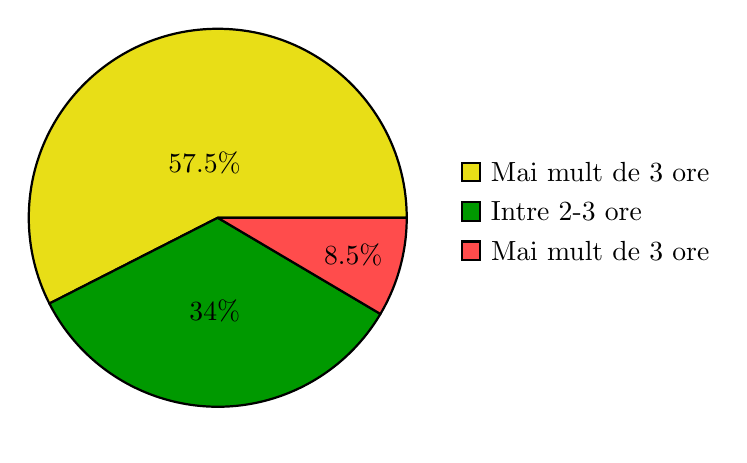
\begin{tikzpicture}[scale=0.8]
					% We will draw the pie chart here
					
					\pie[
					,
					color = {
						yellow!90!black, 
						green!60!black, 
						red!70},
					text = legend
					]
					{57.5/Mai mult de 3 ore,
						34/Intre 2-3 ore,
						8.5/Mai mult de 3 ore}
						  
				\end{tikzpicture}
				\caption{Repartitia respondentilor dupa numarul mediu de ore petrecut online } 
			\end{figure}
		\item Referitor la nivelul de studii absolvit al respondentilor (vezi figura 3.2), esantionul nostru este format  preponderent de absolventi de studii superioare (mai exact 61,3\%), restul fiind în prezent studenți. Mai mult, din tot eșantionul 22,6\% au studii post-universitare.
		\begin{figure}[!htb]
			\centering
			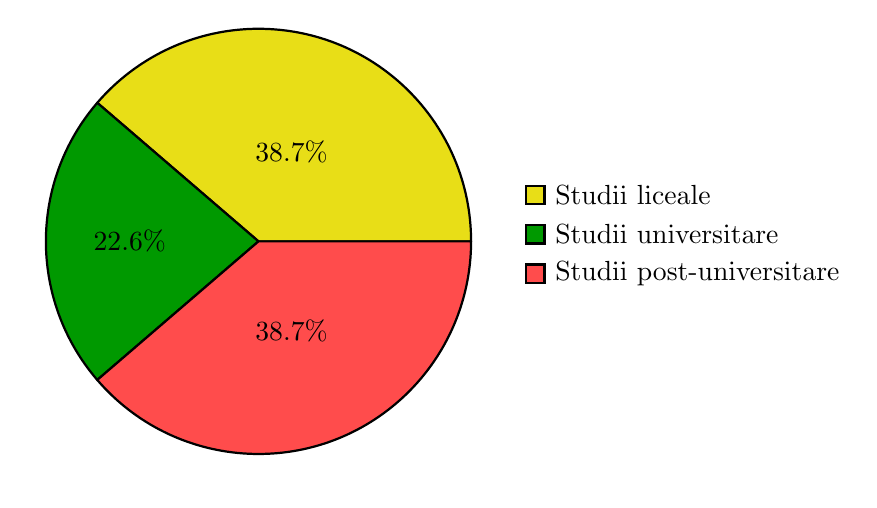
\begin{tikzpicture}[scale=0.9]
				% We will draw the pie chart here
				
				\pie[
				color = {
					yellow!90!black, 
					green!60!black, 
					red!70},
				text = legend
				]
				{38.7/Studii liceale,
					22.6/Studii universitare,
					38.7/Studii post-universitare}
				
			\end{tikzpicture}
			\caption{Repartia respondentilor dupa nivelul de studii absolvit} 
		\end{figure}
		\item Din perspectiva genului, marea majoritate a respondentilor sunt de gen feminin, cu un procent de 90,6\% care indica faptul ca femeile sunt mai empatice pentru a raspunde la chestionare online deoarece studiile analizate anterior nu au indicat nicio diferenta atat de mare intre cele doua sexe, formandu-se un echilibru intre cele doua genuri. Astfel, acest lucru nu inseamna ca barbatii achizitioneaza mai putin in mediul online, deoarece numarul scazut de respondenti de gen masculin reflecta doar o limita a cercetarii noastre si nu o realitate.
		\end{itemize}
	\qquad Pentru urmatoarea parte lucrarii, vom analiza principalele constatări ale
	eșantionarii populației, luând în considerare cele trei obiective definite anterior.
	\begin{enumerate}[(A)]
		\item\textbf{ Primul obiectiv al studiului nostru}: sa identificam ce determina consumatorii online, tineri si educati din Romania sa achizitioneze din mediul online si cum se informeaza.
		
		\qquad Pentru a identifica motivele pentru care cumparatorii prefera sa achizitioneze din mediul online si care este atitudinea lor fata de beneficiile achizitiilor online, am adaugat o intrebare cu 5 itemi de raspuns (Posibilitatea de a realiza comparații, Accesibilitatea 24/24, Oportunitatea de a plăti un preț mai mic, Acces la gama mai larga de produse, Abilitatea de a împărtăși experiențe pe rețelele de socializare), unde respondentii trebuiau sa masoare pe o scara de la 1 la 5 gradul de intensitate al fiecarui item in parte(vezi intrebarea 4 - Anexa 1). Raspunsurile primite sunt reprezentate mai jos(vezi tabelul 3.1).
		\newcolumntype{M}[1]{>{\centering\arraybackslash}m{#1}}
	\bigskip
	\bigskip
					
			\begin{tabular}{ | M{12em} | M{1.2cm}| M{1.0cm} | M{1.2cm}| M{1.2cm} | M{2.2cm} | } 
				\hline
		& \multicolumn{5}{c|}{\textbf{Gradul de acord cu afirmatia }} \\
				\hline
				\centering
				 
				& 1 Deloc & 2      Mic & 3 Mediu & 4 Mare & 5 \qquad Foarte mare \\ 
				\hline
				Posibilitatea de a realiza comparatii & 2,8\% & 10,4\%  & 28,3\% & 22,7\% &35,8\%   \\ 
				\hline
				Accesibilitatea 
				24/24  & 2,8\%  & 0,9\%  & 19,8\% &19,8\%  & 55,7\% \\ 
				\hline
				Oportunitatea de a plăti un preț mai mic & 0,9\% & 6,5\%  &20,8\%  &20,8\% & 51\%  \\ 
				\hline
				Acces la o gamă mai largă de produse &0\%  &4,7\%  & 16\%  & 23,6\% & 55,7\% \\ 
				\hline
				Abilitatea de a împărtăși experiența online &33\%  & 13,2\%  &22,7\%  &16\% &14,1\% \\
				\hline		
			\end{tabular}
	\captionof{table}{Repartiția respondenților după răspunsurile la întrebarea "In ce masura conteaza pentru tine beneficiile achizitiilor online, mentionate mai jos?" } \label{tab:title} 
	\bigskip	

	\qquad Asadar, prin raspunsurile obtinute la aceasta intrebare( vezi Tabelul 3.1.) putem deduce urmatoarele:
	\begin{itemize}
		\item \textit{accesibilitatea 24/24} si \textit{accesul la o gama mai larga de produse}  (ambele detinand un procent de 55,70\%) sunt principalele beneficii pentru care consumatorii online din Romania obisnuiesc sa achizitioneze din mediul online , avantaje ce deosebesc magazinele virtuale de cele traditionale.
		\item Urmatorul beneficiu care a fost ales de catre 51\% dintre respondenti, se refera la \textit{oportunitatea de a plati un pret mai mic} deoarece magazinele online nu au anumite costuri precum chiria spatiului si a utilitatilor, fapt ce reprezinta un mare plus pentru cumparatori.
		\item  Pe de alta parte, cel mai putin important beneficiu al comertului electronic ales de respondenti a fost \textit{abilitatea de a impartasi experienta online}, ceea ce indica faptul ca impartasirea experientei personale nu reprezinta un avantaj al magazinelor virtuale, deoarece consumatorii tineri si educati din Romania isi comunica experientele prin alte metode.
	\end{itemize}
	
	\qquad Pentru a identifica sursele de informare pe care se bazeaza consumatorii online in momentul in care vor sa realizeze achizitii online, am introdus 4 itemi ( Experienta personala, Review-urile de pe site, Opiniile celor apropiati, Informatia oferita de motoarele de cautare), prin care respondentii au putut acorda o nota de la 1 la 5 (in ordine crescatoarea a intensitatii pe care o simte fiecare subiect asupra itemului respectiv)(vezi Intrebarea 5 Anexa 1). Raspunsurile sunt prezentate mai jos(Vezi tabelul 3.2).	
\bigskip
	\newcolumntype{M}[1]{>{\centering\arraybackslash}m{#1}}
	\begin{center}
		
		\begin{tabular}{ | M{13em} | M{1.1cm}| M{1.0cm} | M{1.1cm}| M{1.1cm} | M{2.2cm} |} 
			\hline
			&  \multicolumn{5}{c|}{\textbf{Gradul de acord cu afirmatia} } \\
			
			\hline
			&  1 Deloc & 2 Mic & 3 Mediu & 4  Mare & 5 \qquad Foarte mare\\ 
			\hline
			Experienta personala  & 2,8\% & 1,9\% &10,4\%  & 28,3\% & 56,6\% \\ 
			\hline
			Review-urile de pe site  &0,9\%  &5,7\%   &27,4\%  &39,6\%  &26,4\%\\ 
			\hline
			Opiniile celor apropiati & 3,7\% & 3,7\%  & 29,2\%  & 35,8\% & 26,4\% \\ 
			\hline
			Informatia oferita de motoarele de cautare & 9,4\% &10,4\%  &34,9\%  &34,9\% & 10,4\% \\ 
			\hline
		\end{tabular}
	\captionof{table}{Repartiția respondenților după răspunsurile la întrebarea "In ce masura esti in
uentat de factorii de mai jos atunci cand realizezi achizitii online? "} \label{tab:title} 
	\bigskip
		
	\end{center}
	\qquad Conform datelor culese, in momentul achizitiei unui produs online, consumatorii se bazeaza cel mai mult pe\textit{ experienta personala} din trecut, detinand cel mai mare procent (84,9\%),urmand apoi cu un procent de 66\% \textit{review-urile de pe site}. Acest fapt denota un aspect neasteptat si anume o incredere mai mare asupra review-urilor online decat in opiniile celor apropiati, ce poate fi explicat prin obiectivatea de care vor sa dea dovada tinerii cumparatori. Cel mai mic procent (45,3\%) l-a obtinut informatia oferita de motoarele de cautare,acest lucru putand fi datorat fie volumului mare de date disponibile online, fie gradului scazut de acuratete a informatiei prezente pe internet.
	
	\qquad Pentru a identifica elementele care conteaza cel mai mult pentru consumator atunci cand ia decizia de a alege un magazin online in detrimentul altuia, am introdus o intrebare cu 5 itemi(Brand-ul produsului, Usurinta utilizarii site-ului, Politica de Return, Diversitatea gamei de produse, Posibilitatea de a urmari comanda realizata), prin care respondentii au putut acorda o nota de la 1-5 in ordinea crescatoare a intensitatii pe care o simte fiecare subiect asupra item-ului respectiv(vezi intrebarea 6 Anexa 1). Raspunsurile sunt prezentate mai jos.(vezi tabelul 3.3)
\bigskip
	\newcolumntype{M}[1]{>{\centering\arraybackslash}m{#1}}
		\begin{center}
		\begin{tabular}{ | M{12em} | M{1.1cm}| M{1.0cm} | M{1.1cm}| M{1.1cm} | M{2.2cm} |} 
			\hline
			& \multicolumn{5}{c|}{\textbf{Gradul de acord cu afirmatia} } \\
			\hline
			& 1 Deloc & 2 Mic & 3 Mediu & 4  Mare & 5 \qquad Foarte mare\\ 
			\hline
			 Brand-ul produsului &1,9\%  &10,4\%  & 41,5\%  &21,7\% &24,5\% \\ 
			\hline
		     Usurinta utilizarii site-ului& 3,8\% & 3,8\%   &17\%  &37,7\%  &37,7\% \\ 
			\hline
			Politica de Return & 5,7\%  &9,4\%  &18,9\%  &33\% &33\% \\ 
			\hline
			Diversitatea gamei de produse & 0,9\%  &2,8\%  &13,2\%  &33\% &50\% \\ 
			\hline
			Posibilitatea de a urmari comanda realizata & 2,8\%  & 6,6\%  &18,9\%  &32,0\% &39,6\% \\
			\hline
		\end{tabular}
	\captionof{table}{Repartiția respondenților după răspunsurile la întrebarea "In ce masura conteaza elementele enumarate mai jos atunci cand alegi un magazin online?" } \label{tab:title} 
	\bigskip
		
		\end{center}
		\qquad Potrivit raspunsurilor primite, am obtinut urmatoarele rezultate:
		\begin{itemize}
			\item Jumatate din totalul de respondenti au oferit grad maxim item-ului privind \textit{diversitatea gamei de produse}, acesta avand si cel mai mare procent (83\%), rezultat ce denota atractia cumparatorului online tanar si educat fata de un magazin mixt  in locul unuia specializat pe o singura gama de produse. Acest lucru se datoreaza faptului ca procesul de achizitie a consumatorului se simplifica, acesta avand posibilitatea de a cumpara mai multe produse dintr-un singur loc si dovedind abilitati de organizare si eficientizare a achizitiilor.
			\item Pe urmatorul loc, cu procentul de 75,4\%, este \textit{usurinta utilizarii site-ului} element ce determina importanta nivelului de accesibilitate al paginii web pentru consumatorii tineri si educati care obisnuiesc sa achizitioneze online cele mai bune oferte gasite.
			\item Un alt aspect interesant este faptul ca \textit{Politica de return }are un scor mediu (66\%), fapt ce pune la indoiala informatiile pe care le au consumatorii tineri si educati cu privire la drepturile lor privind returnarea bunurilor achizitionate. 
			\item De asemenea, contrar asteptarilor, elementul cu cele mai putine voturi il reprezinta \textit{brand-ul produsului} avand un procent de doar 46,2\%, care indica faptul ca, in prezent, consumatorii online nu mai pun cel mai mare accent pe notorietatea  magazinului de la care cumpara, ci se focuseaza pe alte elemente in procesul decizional, precum cele amintite anterior.
		\end{itemize}
		
		\quad Referitor la nivelul de documentare a consumatorilor inaintea plasarii unei comenzi online, am introdus o intrebare cu un singur item prin care respondentii au putut acorda o nota de la 1 la 5 in ordinea crescatoare a intensitatii cu care se informeaza.
		
		\begin{figure}[!htb]
			\centering
			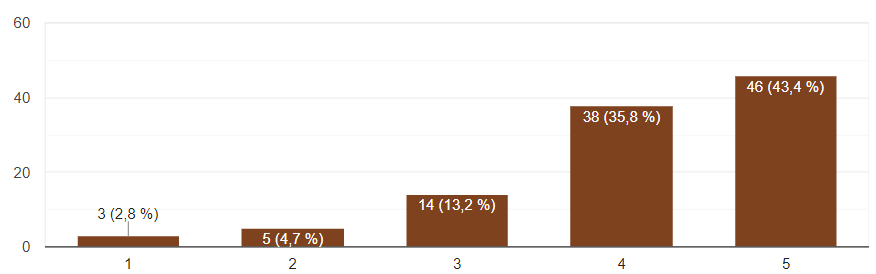
\includegraphics[width=14cm, height=5cm]{"figures/trei.png"}
			\caption{ Repartizarea respondentilor dupa nivelul de documentare a respondentilor inainte de a comanda online}\label{fig:unuspre}
		\end{figure}
	
	 	\qquad Asadar, prin raspunsurile oferite se observa ca respondentii  au un nivel crescut de maturitate, alegand sa se informeze riguros inainte de a alege sa cumpere un produs, deoarece  35,8\% au ales ca se informeaza mult, iar 43,4\%, aproape jumatate, au ales chiar grad maxim de informare. Acest lucru este subliniat si de faptul ca doar 2,8\% din respondenti au ales cea mai mica nota (1) care inseamna informare deloc. Astfel, se observa o crestere a nivelului de educatie al consumatorilor tineri si educati din Romania prin atentia pe care o ofera cumparaturilor in mediul online.

	 	
		\item \textbf{Al doilea obiectiv al studiului nostru }: sa identificam categoriile de produse si frecventa achizitiilor online.
		
		\quad Pentru a identifica categoriile de produse cele mai achizitionate in mediul online, am propus acestora sa raspunda care e categoria de produse pe care o cumpara cel mai des online.(vezi intrebarea 7 Anexa 1).
		\begin{figure}[!htb]
			\centering
			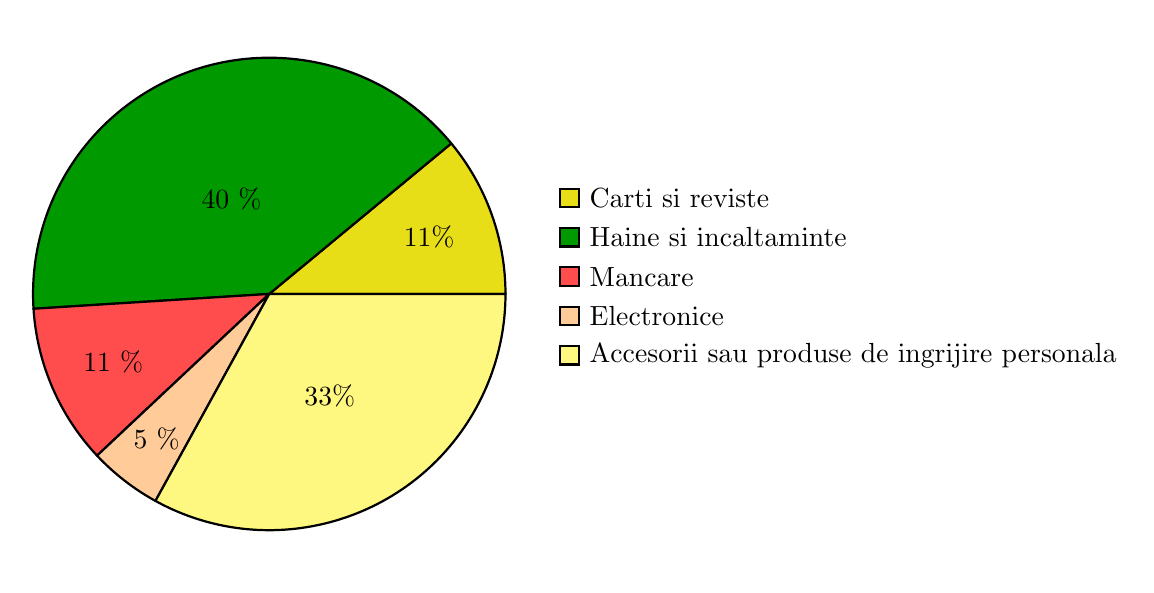
\begin{tikzpicture}
				% We will draw the pie chart here
				
				\pie[
				color = {
					yellow!90!black, 
					green!60!black, 
					red!70,
					orange!40,
					yellow!50 },
				text = legend
				]
				{11/Carti si reviste,
					40 /Haine si incaltaminte,
					11 /Mancare,
					5 /Electronice,
					33/ Accesorii sau produse de ingrijire personala}
				
			\end{tikzpicture}
			\caption{Repartitia respondentilor dupa categoria cea mai achizitionata in perioada feb-april 2021} 
		\end{figure}
	
		\quad Cei mai multi dintre respondenti ( vezi figura 3.4) au raspuns ca\textit{ hainele si incaltamintea} reprezinta cea mai frecventa categorie de produse achizitionata. Pe locul doi se afla \textit{accesoriile/ produsele de ingrijire personala}, iar pe trei,\textit{ cartile si revistele} aflandu-se la egalitate cu \textit{mancarea}. Aceste categorii de produse au fost bunurile care au fost cele mai importante pentru consumatorii online, tineri si educati din Romania in perioada februarie-aprilie 2021.
	
		\qquad Pentru a cunoaste frecventa  cu care consumatorii achizitioneaza, in mediul  online, am propus acestora sa raspunda cat de frecvent obisnuiesc ei sa achizitioneze produse sau servicii cu ajutorul internetului fie de pe laptop/telefon sau tableta(vezi intrebarea 8, Anexa 1)
		\begin{figure}[!htb]
			\centering
			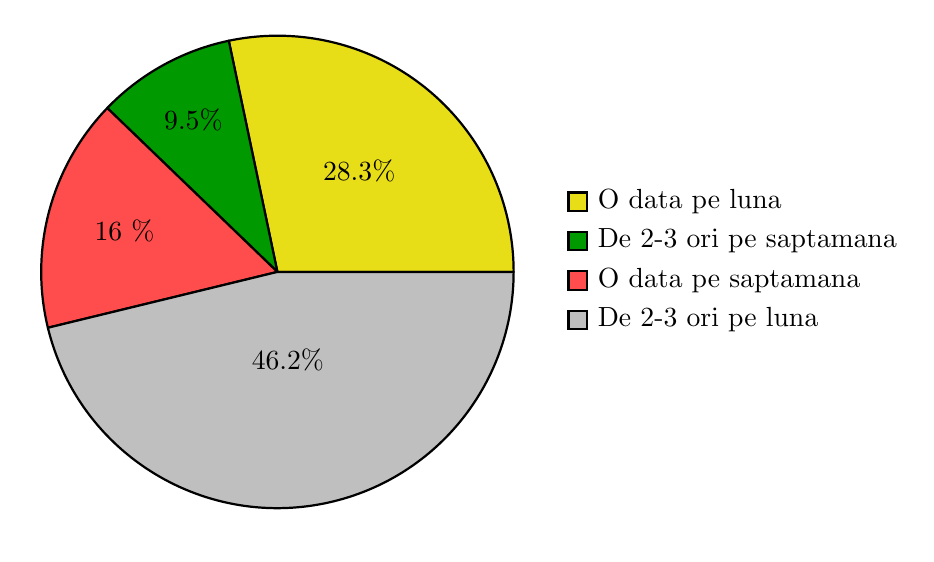
\begin{tikzpicture}
				% We will draw the pie chart here
				
				\pie[
				color = {
					yellow!90!black, 
					green!60!black, 
					red!70,
					gray!50},
				text = legend
				]
				{28.3/O data pe luna,
					9.5/De 2-3 ori pe saptamana,
					16 /O data pe saptamana,
					46.2/De 2-3 ori pe luna}
				
			\end{tikzpicture}
			\caption{Repartitia respondentilor dupa categoria cea mai achizitionata in perioada februarie-aprilie 2021} 
		\end{figure}
	
\newpage
		\qquad Conform raspunsurilor culese,(vezi Figura 3.5) cei mai multi respondenti (46,2\%) au spus ca achizitioneaza de \textit{2-3 ori pe luna}, fapt ce se incadreaza ca o medie intre des si rar, iar cei mai putini respondenti (9,4\%) au spus ca achizitioneaza de \textit{2-3 ori pe saptamana}.
\bigskip	
		\item \textbf{Al treilea obiectiv al studiului nostru}: Sa identificam problemele aparute si comportamentul post-achizitie al consumatorilor online tineri si educati din Romania.
\end{enumerate}		
		\quad Pentru a afla ce tip de probleme au intampinat atunci cand au achizitionat un produs online, am adaugat o intrebare cu 5 itemi (Timpul de livrare nu a fost respectat, Produsul a ajuns cu defecte, Au fost costuri mari cu livrarea, Calitate inferioara, Returnarea produsului a fost dificila) prin care respondentii au putut acorda o nota de la 1-5 in ordinea crescatoare a intensitatii pe care o simte fiecare subiect asupra item-ului respectiv(vezi intrebarea 10, Anexa 1). Raspunsurile sunt prezentate mai jos(vezi tabelul 3.4).
	\newline
	
\bigskip		
		\newcolumntype{M}[1]{>{\centering\arraybackslash}m{#1}}
		\begin{center}
			\begin{tabular}{ | M{14em} | M{1.1cm}| M{1.0cm} | M{1.1cm}| M{1.1cm} | M{2.2cm} |} 
				\hline
				& \multicolumn{5}{c|}{\textbf{Gradul de acord cu afirmatia} } \\
				\hline
				& 1 Deloc & 2 Mic & 3 Mediu & 4  Mare & 5 \qquad Foarte mare\\ 
				\hline
				Timpul de livrare nu a fost respectat  &8,5\%  &37,7\%  &27,4\%  &18,9\% &7,5\% \\ 
				\hline
				Produsul a ajuns cu defecte &34\%  &44,3\%   &17\%  &4,7\%  &0\%\\ 
				\hline
				Au fost costuri mari cu livrarea &13,2\%  & 26,4\%  &29,2\%  &18,9\% &12,3\% \\ 
				\hline
				Calitate inferioara &18,9\%  &41,5\%  & 24,5\%  &12,3\%  &2,8\% \\ 
				\hline
				Returnarea produsului a fost dificila & 32,6\%  & 27,4\%  & 18\% & 9,4\% &5,7\% \\
				\hline
			\end{tabular}
		\captionof{table}{Repartiția respondenților după răspunsurile la întrebarea "In ce masura ati intampinat problemele de mai jos atunci cand ati comandat un produs de pe internet?" } \label{tab:title} 
		
		\end{center}
	\qquad\space\space Potrivit datelor culese(vezi tabel 3.4), consumatorii online tineri si educati nu au prea intalnit acest tip de probleme atunci cand au plasat o comanda online, fapt dovedit de notele mici acordate problemelor din figura de mai sus. Cea mai intalnita, dar care tot detine un scor nu foarte mare (31,2\%) este \textit{costuri mari cu livrarea}, urmand pe locul doi, cu un procent de 26,4\%, \textit{timpul de livrare care nu a fost respectat} fapt ce subliniaza importanta calitatii livrarii bunurilor in procesul de achizitie online. Problema intalnita cel mai putin a fost \textit{Produsul a ajuns cu defecte} avand un procent de aproape 5\%.
	
	\quad Pentru a identifica cum reactioneaza consumatorii  online atunci cand intalnesc o problema cu produsul livrat de la un magazin online, am intrebat cum au actionat ei dupa ce au constat ca bunul primit in urma comenzii, nu este conform cerintelor lor. Raspunsurile sunt prezentate mai jos(vezi figura 3.6).
	\begin{figure}[!htb]
		\centering
		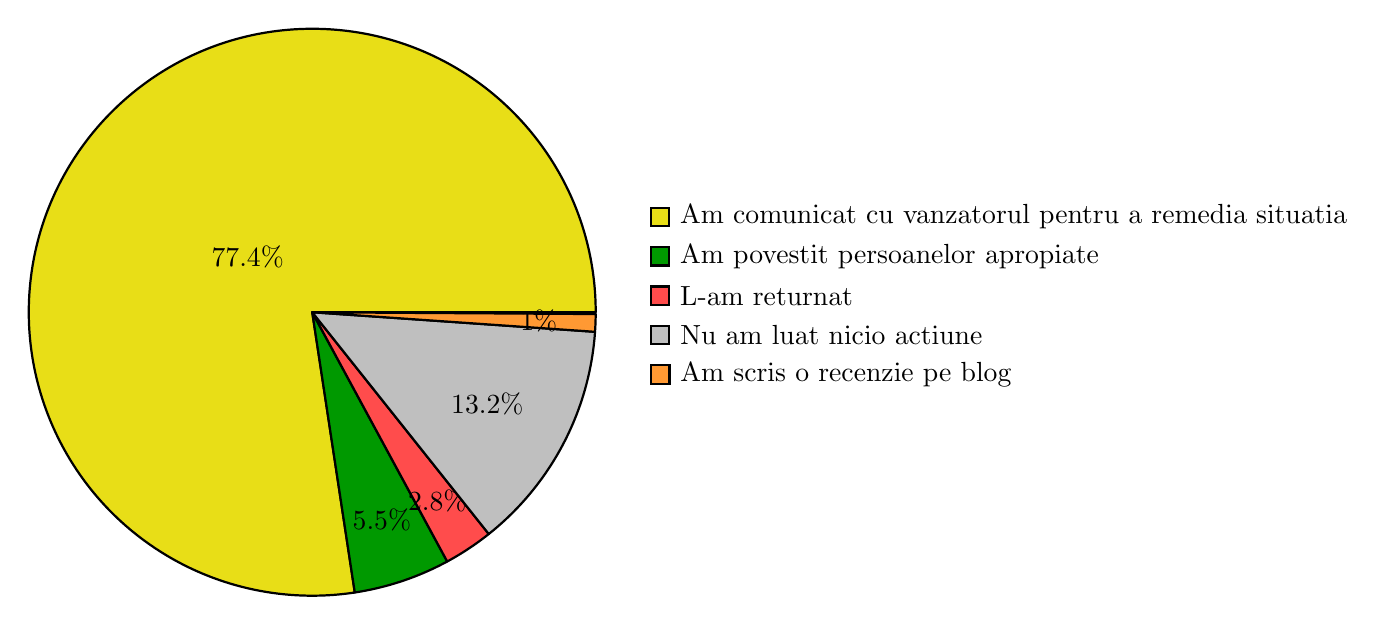
\begin{tikzpicture}[scale=1.2]
			% We will draw the pie chart here
			
			\pie[
			color = {
				yellow!90!black, 
				green!60!black, 
				red!70,
				gray!50,
				orange!80},
			text = legend
			]
			{77.4/Am comunicat cu vanzatorul pentru a remedia situatia,
				5.5/Am povestit persoanelor apropiate,
				2.8/L-am returnat,
				13.2/Nu am luat nicio actiune,
				1/Am scris o recenzie pe blog}
			
		\end{tikzpicture}
		\caption{Repartitia respondentilor dupa problemele pe care le-au intalnit in achizitia unor produse online} 
	\end{figure}

	\quad Conform raspunsurilor obtinute, am constat ca cei mai multi respondenti, anume un procent de 77,4\% din total au raspuns ca ei comunica problema intalnita vanzatorului/ magazinului de la care a achizitionat bunul pentru a putea remedia si rezolva situatia creata, fapt ce subliniaza inca o data seriozitatea si increderea de care da dovada consumatorul online si tanar fata de achizitiile din mediul online. Acest lucru evidentiaza profilul stabilit al participantilor, la acest studiu, inca de la inceputul cercetarii. Din pacate, au existat si persoane (13,20\%) care au ales sa nu ia nicio actiune cu privire la bunul achizitionat si neconform cerintelor si asteparilor lor. Au existat si cateva pareri, in minoritate, care au ales sa actioneze diferit si unic precum: impartasirea experientei celor apropiati(5,5\%), returnarea produsului (2,8\%) si scrierea experientei pe un blog (0,9\%).
	
	\quad In ultima parte a analizei datelor culese doresc sa integrez intrebarile deschise de la finalul chestionarului (vezi intrebarea 12 si 13, Anexa 1) alaturi de celelalte intrebari pentru a crea un profil al respondentilor bazat pe cele 3 categorii de varsta (18-21, 22-24, 25-30) si pentru a putea identifica diferentele ce pot aparea intre segmentele de clienti, in functie de categoria de varsta. 
	
	\quad In cadrul intrebarile deschise, privind experientele consumatorilor, am dorit sa vedem ce considera  el ca fiind cea mai buna experienta in mediul online si problemele care l-au determinat sa vada o alta experienta, drept cea mai putin buna.
	
	\quad Din cauza faptului ca predomina respondentii de gen feminin cu peste 90\% din esantion, voi analiza in continuare raspunsurile primite de la consumatorii online de gen feminin.
	
	\quad Faptul ca procentul raspunsurilor feminine excede procentul raspunsurilor masculine poate indica faptul ca femeile sunt mai empatice la raspunderea de chestionare online decat barbatii sau poate fi datorat implicarii unui numar restrans de respondenti de gen masculin in completarea chestionarului.

	\quad Din procentul de 90,6\% din totalul persoanelor care au raspuns la chestionar, 33\% dintre respondentii de gen feminin au varsta cuprinsa intre 18-21 de ani( abia au terminat studiile liceale sau sunt studente la o facultate), 29\% au varsta cuprinsa intre 22-24 ( sunt absolvente de licenta sau studente la master), 38\% au varsta cuprinsa intre 25-30 de ani (fie sunt absolvente de studii superioare sau studente la doctorat)(vezi figura 3.7).
	\begin{figure}[!htb]
		\centering
		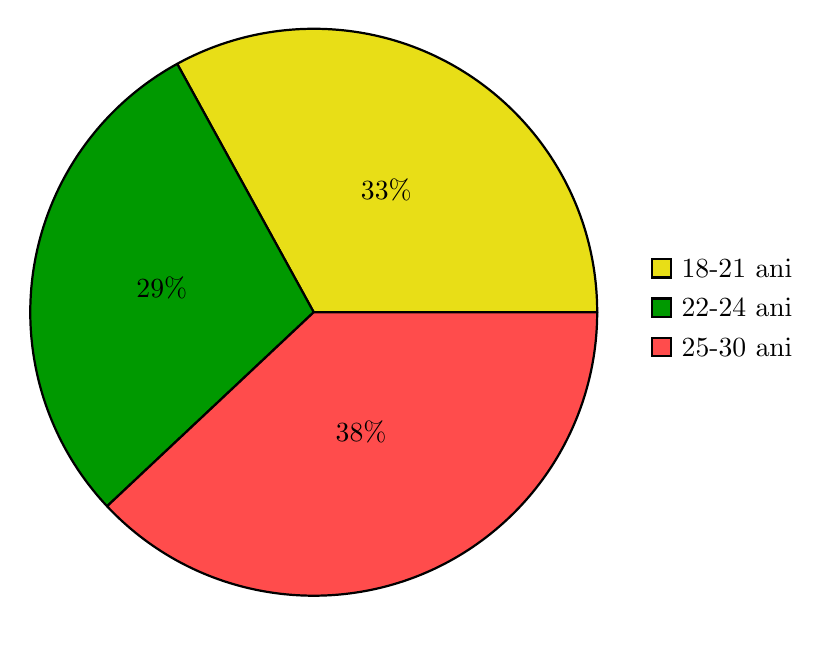
\begin{tikzpicture}[scale=1.2]
			% We will draw the pie chart here
			
			\pie[
			color = {
				yellow!90!black, 
				green!60!black, 
				red!70},
			text = legend
			]
			{33/18-21 ani ,
				29/22-24 ani,
				38/25-30 ani}
			
		\end{tikzpicture}
		\caption{Repartitia respondentilor dupa problemele pe care le-au intalnit in achizitia unor produse online} 
	\end{figure}
\newpage		
	\begin{itemize}
		\item \textbf{Prima categorie de varsta (18-21 ani)} reprezinta 33\% din totalul de respondenti de gen feminin. In  urma analizei asupra datelor oferite, am extras informatiile relevante pentru a putea sublinia caracteristicile acestei categorii. 
		
		\quad Primul lucru pe care l-am sesizat a fost faptul ca 57\% dintre respondentii acestei categorii petrec mai mult de 3 ore online, inafara cursurilor de la facultate, insa frecventa cu care comanda online este redusa, procentul de  37\% spunand ca plaseaza comenzi o data pe luna . Acest lucru releva un paradox si anume, daca o persoana petrece mult timp in mediul online nu inseamna ca isi face cumparaturile tot in acest mediu.
		
		\quad Urmatorul lucru pe care l-am identificat a fost faptul ca\textit{ hainele si incaltamintea} reprezinta cea mai frecventa categorie de produse achizitionata online (50\% au ales aceasta categorie),  fapt ce releva increderea pe care o au acesti consumatori tineri in aceste magazine. Acest lucru este subliniat si de procentul ridicat de 68,8\% in care acestia au raspuns ca atunci cand apar eventuale erori cu comanda sau produsul achizitionat au siguranta ca pot comunica cu producatorul pentru a remedia situatia ulterior. 
		
		\quad Pentru a analiza raspunsurile oferite de respondenti la intrebarile deschise am decis sa grupam experientele impartasite pentru a le evidentia pe cele care s-au afirmat cel mai mult:
		\begin{itemize}
			\item In cazul intrebarii deschise referitoare la cea mai buna experienta pe care au avut-o pana acum, consumatorii au subliniat in mare parte avantajele pe care magazinele online le ofera cumparatorilor si care conteaza cel mai mult pentru ei. Dintre acestea enumeram: rapiditatea livrarii produsului intr-un timp cat mai scurt, fiind cel mai des mentionat element, urmand apoi disponibilitatea producatorului de a raspunde si remedia eventuale erori si apoi posibilitatea de a urmari produsul achizitionat in timp real.
			\item 	In cadrul intrebarii referitoare la experienta mai putin buna s-au accentuat problemele pe care consumatorii le-au intalnit. Dintre acestea, cel mai mult s-au mentionat timpul de livrare care nu a fost respectat si neconcordanta dintre calitatile promise in mediul online fata de cele primite la momentul livarii produsului. 
		\end{itemize}
		\item \textbf{A doua categorie de varsta (22-24 ani)} este reprezentata de 29\% din totalul de respondenti de gen feminin. In aceasta categorie s-au sesizat mici diferente, fata de cea analizata anterior pe care le voi prezenta in randurile urmatoare.
		
		\quad Prima diferenta pe care am sesizat-o la femeile e-consumator, cu varsta cuprinsa intre 22-24, este ideea ca in ciuda faptului ca petrec tot la fel de mult timp online ca si generatia anterioara, procentul de achizitii online cel mai mare (60\%) este la varianta cu 2-3 achizitii pe luna. Acest fapt ne indica ca femeile sunt mult mai atente cu programul lor si ca incearca sa-si organizeze cat mai eficient activitatile ce necesitau ore inainte in magazinele fizice, dar posibile doar cu un click in mediul online.
		
		\quad Urmatoarea diferenta pe care am observat-o a fost la categoriile de produse achizitionate cel mai des online. Fata de generatia anterioara, respondentii de gen feminin din aceasta categorie au un procent mai scazut (42,9\%) la categoria de \textit{haine si incaltaminte}, urmat de \textit{accesorii si produse de ingrijire} cu un procent de 35,8\%. Acest lucru dezvaluie tendinta fetelor de a pune mult mai mare accent pe ingrijirea personala cu inaintarea in varsta. 
		
		\quad La intrebarile deschise aflate la finalul chestionarului, fetele au mentionat aproximativ aceleasi elemente care s-au amintit, referitoare la experientele pozitive si negative pe care le-au avut, in schimb, s-au sesizat cateva elemente de noutate precum:
		\begin{itemize}
			\item In cadrul celei mai bune experiente s-a adaugat cererea de feedback din partea producatorului, existenta unor costuri mai mici online si utilizarea site-urilor pentru comparatii intre produsele dorite drept elemente care ajuta la incheierea cu succes a unui proces de achizitionare in mediul electronic.
			\item In cazul experientei mai negative s-a adaugat lipsa returnarii sumei oferite pe achizitionarea produsului in urma returnarii acestuia, fapt ce constituie o mare problema in randul consumatorilor de orice gen.
		\end{itemize}
	
		\item \textbf{Ultima categorie de varsta (25-30 ani)} reprezinta cel mai mult din totalul de respondenti de gen feminin si anume 38\%. In cadrul acestei analize am facut o comparatie intre cele doua generatii prezentate anterior si generatia care a devenit matura si trebuie sa ofere mai multe atentie costurilor pe care le are.
		
		\quad In primul rand, persoanele de gen feminin cu varsta intre 25 si 30 de ani petrec la fel de mult timp online, acest lucru putand fi datorat job-ului care s-a transformat remote in contextul pandemiei Covid19, insa achizitioneaza mai mult decat prima categorie de varsta, ceea ce releva o stabilitate materiala dar mai putin decat a doua, fiind mult mai atente pe ce cheltuiesc banii castigati din venituri proprii.
		
		\quad In al doilea rand, fetele/femeile din acest grup subliniaza tendinta pe care am observat-o si la generatia anterioara privind accentul pe \textit{produsele de ingrijire personala} cu un procent de 43,5\%, iar locul 2 fiind ocupat, in acest caz, de categoria de \textit{haine si incaltaminte}. De asemenea, noua categorie de produse (electrocasnicele)  introdusa de acestia si procentul mare (69,5\%) obtinut in vederea comunicarii cu producatorul indiferent de problemele intalnite, releva o nota de maturitate venita odata cu cresterea in varsta.
		
		\quad In ultimul rand, experientele dezvaluite la intrebarile deschise au expus noi caracteristici/elemente pe care consumatorii le doresc sa le intalneasca sau nu precum:
		\begin{itemize}
			\item Elementele dorite si care vin in completarea celorlalte experiente pozitive, amintite anterior, sunt suprizele sau produsele extra pe care unii producatori le folosesc pentru a-si loializa clientii si  calitatea ridicata unor produse importante si vitale precum o piesa auto ce dupa spusele unei respondente a rezistat conform trasaturilor mentionate.
			\item Elementele care se doresc a fi evitate sunt reprezentate costurile mari cu transportul si nerespectarea timpului de livrare, insa in cazul acestui interval de varsta, aceste achizitii au fost efectuate inafara tarii, fapt ce ingreuneaza procesul de achizitie si livrare datorita taxelor vamale si distantei foarte mari dintre producator si destinatar.
		\end{itemize}
	\end{itemize}
\newpage	
	\subsection{Concluzii - studiu de caz}
	\qquad In urma cercetarii realizate, avem un profil al comportamentului consumatorului online, tanar si educat din Romania avand in vedere elementele de care are nevoie pentru a achizitiona mai mult in mediul online dar si trasaturi negative care inca nu-i ofera siguranta de a utiliza comertul electronic.
	concluzionam urmatoarele :
	\begin{enumerate}[1.]
	\item Cele mai importante beneficii ale comertului electronic evidentiate de respondenti sunt accesibilitatea 24/24 si livrarea rapida a produselor alaturi de accesul la o gama mai larga de produse la preturi mai avantajoase decat in magazinele fizice.
	\item Experienta personala reprezinta sursa de baza in momentul in care un consumator tanar, educat decide sa-si achizitioneze un produs din mediul online, fapt ce suprinde datorita existentei unui volumul mare de informatii disponibil pe motoarele de cautare, dar care, din pacate, reprezinta ultima sa sursa de informare din diverse precum autenticitatea informatiilor disponibile, sursele de informare nu sunt adesea actualizate prezentului iar detaliile de pe site nu pot fi intotdeauna verificate.
	\item Motivul pentru care unii consumatori, tineri si educati din Romania aleg un magazin electronic in detrimentul altuia este diversitatea gamei de produse, care ajuta consumatorii online romani sa-si eficientizeze productivitatea folosind un clik de pe un singur site.
	\item Legat de masura in care se documenteaza consumatorii online tineri si educati inainte de a plasa o comanda, respondentii au evidentiat nivelul de educatie crescut prin acordarea notei maxime, care inseamna ca sunt mult mai atenti cu produsele pe care le achizitioneaza si de unde le cumpara inainte de a plati
	\item In ciuda faptului ca pandemia covid19 a restrictionat accesul persoanelor in magazine si supermarket-uri, categoria de produse cea mai achizitionata online nu este mancarea, ci hainele si incaltamintea, iar acest fapt se datoreaza gamei largi de produse de imbracaminte ce poate fi gasita in magazinele virtuale si codurilor de reducere care se pot utiliza exclusiv online.
	\item Analizand proportionalitatea dintre timpul petrecut online si frecventa achizitiilor online am constat ca nu exista o regula stabila care sa functioneze deoarece am intalnit in cadrul rezultatelor persoane care petreceau mult timp online, insa numarul de achizitii depindea de categoria de varsta in care se incadra respondentul.
	\item S-a evidentiat drept cea mai importanta problema, costurile si timpul livrarii produsului care nu ingreuneaza satisfacerea nevoilor cumparatorilor. De asemenea, respondentii au afirmat ca atunci cand intampina probleme cu produsul achizitionat si livrat acasa, ei decid sa comunice cu producatorul pentru a putea remedia situatia in cel mai scurt timp posibil.
	\end{enumerate}
	
	\quad Profilul socio-demografic al consumatorilor online, tineri si educati din Romania participanti la sondajul de opinie realizat (esantionul fiind de 106 persoane) este: majoritatea sunt persoane de gen feminin (90,6\%). In randul respondentilor, 31,1\% au varsta cuprinsa intre 18-21 ani, 25,5\% au varsta cuprinsa intre 22-24 de ani, iar 26,4\% au varste cuprinse intre 25-30 de ani. Majoritatea respondentilor chestionati sunt absolventi de studii superioare de nivel licenta sau masterat sau studenti ai acestor programe. 
	
	

	
	\newpage 
	\section*{Concluzii}
	\addcontentsline{toc}{section}{\textsc{Concluzii }}
	
	\qquad Tema acestei lucrari "Comportamentul consumatorului online tanar si educat din Romania. Studiu de caz" este abordata pe parcursul celor 3 capitole care cuprind informatii in general despre comportamentul unui consumator online, in general si in particular comportamentului consumatorului online tanar si educat din Romania. De asemenea, este abordat specificul comertului electronic, atat la nivel conceptual, cat si la nivel de Uniune Europeana dar si situatia din Romania. La nivelul studiului de caz scopul urmarit a fost crearea unui profil al consumatorului online tanar si educat din Romania pentru a ajuta firmele din comertul electronic sa inteleaga mai bine comportamentul acestuia si sa se plieze pe cerintele lui.
	
	\quad Prima parte a lucrarii studiaza, in ansamblul, comertul electronic si procesul decizional al consumatorului online. Comertul electronic s-a dezvoltat din ce in ce mai mult in ultimii ani, iar acest lucru a fost evidentiat prin faptul ca acesta devenit o componenta importanta a sistemului de afaceri. De asemenea, comertul electronic cuprinde atat tranzactii cu bunuri tangibile, cat si tranzactii privind bunurile intangibile. Astfel, consumatorii online au oportunitatea de a alege dintr-o gama mai larga de optiuni oferite de magazinele digitale, iar managerii au oportunitatea de a analiza informatiile oferite de consumator, transformand aceste date direct in strategii de marketing. Avand in vedere multitudinea de posibilitati care i se ofera cumparatorului, in mediul virtual, acesta este nevoit sa ia in considerare anumite elemente mai importante pentru achizitionarea unui produs in detrimentul altuia. Acesti factori i-am putea imparti in doua categorii: factori ce tin de persoana consumatorului precum constrangerile de timp, motivatia cumpararii, nivelul de informare si factori ce tin de magazinul digital precum accesibilitatea site-ului, securitatea informatiilor, calitatea oferita de magazin si altele. Procesul de cumparare al consumatorului online nu se diferentiaza cu mult de cel al consumatorului fizic deoarece la baza exista acelasi etape, doar cu mentiunea ca acestea au loc exclusiv online. Cumparatorul acum va cauta informatia online cu ajutorul motoarelor de cautare si va apela mult mai usor la review-uri. Va putea compara si analiza informatia utilizand instrumente de sortare si filtrare a datelor, iar luarea deciziei va avea loc numai dupa ce consumatorul este constient de riscurile posibile. In cazul mediului online, mecanismul de reclamatii poate fi un proces mult mai greu, unii utilizatori alegand sa nu mai remedieze situatia cu producatorul.Interactiunile post-vanzare sunt facilitate de mediul online, oferind posibilitatea de loializare a clientilor prin email-uri de promovare. La fel ca orice alt proces, achizitionarea de produse online are si ea avantajele si dezavantajele ei. Avantajul cel mai important il reprezinta accesul la o varietate mai larga de produse, iar cel mai mare dezavantaj este livrarea unui produs cu o calitate inferioara.
	
	\quad Prezenta lucrare continua cu o cercetare secundare asupra situatiei din Romania privind achizitiile online si comportamentul consumatorului online tanar si educat. Piata de comert electronic din Romania este in stransa legatura cu accesul la Internet, iar avand in vedere ca rata de penetrare pe Internet era scazuta fata de media Uniunii Europene, mediul online este accesat doar de o parte din populatie, fapt ce ingreuneaza dezvoltarea comertului  in mediul digital. Datorita cresterii nivelului de educatie, s-a dovedit ca noua generatie de tineri este mult mai familiarizata cu tehnologia online si este mai dispusa sa se confrunte cu riscurile percepute de mediul virtual. Cele mai achizitionate categorii de produse de romanii care achizitioneaza online sunt electronicele, imbracamintea si produsele de frumusete si ingrijire personala. Un alt factor care a influentat dezvoltarea comertului electronic in Romania este pandemia Covid19, care a dus la o crestere a cumparaturilor online in randul romanilor. In acest capitol am realizat si o comparatie intre trei cercetari care au abordat tema comportamentului consumatorului online din Romania intr-un mod unic. Prima cercetare a evidentiat dezvoltarea comertului electronic prin extinderea inafara granitelor tarii. A doua cercetare a abordat tulburarea de cumparare compulsiva care a rezultat ca este mai evidentiata la femei. Ultima cercetare a subliniat toate avantajele si dezavantajele cumparaturilor online.
	
	\quad Studiul de caz al acestei lucrari se gaseste in cadrul celui de-al treilea capitol, cuprinzand o analiza ce releva motivele pentru care cumparatorii online, tineri si educati din Romania cumpara din mediul digital, ce categorii de produse achizitioneaza si cum reactioneaza la problemele aparute. Scopul acestui studiu de caz este realizarea profilului consumatorului online tanar si educat din Romania pentru a oferi informatii firmelor prezente in mediul online care tintesc acest tip de consumator in strategiile lor. Studiul de caz are la baza o cercetare primara cantitativa, metoda folosita fiind sondajul de opinie. Instrumentul folosit a fost chestionarul lansat online prin intermediul aplicatiei Google Forms avand un numar de 106 raspunsuri valide.
	
	\quad Datele obtinute in urma cercetarii coincid cu notiunile teoretice formulate pe baza surselor bibliografice si a studiilor efectuate anterior. Notiunile teoretice au fost dezvoltate pe parcursul celor doua capitole anterioare si servesc drept premise in desfasurarea studiului.
	
	\quad Concordanta dintre notiunile teoretice analizate pe parcursul celor 2 capitole si datele obtinute in urma cercetarii este vizibila. Astfel, potrivit datelor culese in urma interviului lansat concluzionam ca anumite aspecte privind comportamentul consumatorului online tanar si educat din Romania s-au pastrat de-a lungul dezvoltarii comertului electronic precum motivul pentru care aleg sa achizitioneze si anume oportuntiatea unei game mai largi de produse, alegerea unui produs in urma experientei personale si nu a opiniilor altor consumatori online, cea mai achizitionata categoria de produse online a ramas tot imbracamintea si incaltamintea. De asenmenea, exista si anumite aspecta care s-au schimbat si imbunatatit precum cresterea nivelului de informare inainte de a cumpara un produs online, fapt ce releva statutul educationat ridicat, iar acest lucru este subliniat si de comportamentul responsabil al consumatorului online tanar si educat care alege sa discute cu producatorul pentru a remedia problemele ce apar.
	
	\quad Concluzionand subiectul tratat pe parcursul acestor pagini il putem descrie ca fiind unul complex si de actualitate si in acelasi timp interesant si inovat pentru domeniul marketing-ului online. Urmarirea modului in care se dezvolta comportamentul consumatorului online tanar si educat din Romania in concordanta cu dezvoltarea comertului electronic ramane un subiect instigator ce aduce in permanenta noi oportunitati de cercetare si asta deoarece companiile doresc identificarea si satisfacerea nevoilor consumatorilor online in asa fel incat acestia sa fie atrasi cat mai mult in a cumpara online.
	\newpage
	
	
\newpage 
\bibliographystyle{unsrt}
\bibliography{references}

\newpage 
	\section*{Anexa 1- Chestionarul Comportamentul consumatorului online, tanar si educat din Romania }	
\addcontentsline{toc}{section}{\textsc{Anexa 1- Chestionarul Comportamentul consumatorului online, tanar si educat din Romania }}
	\quad Bună ziua! Mă numesc Ciucanu Elena-Sorina, sunt studentă în anul III la Management, FSE, UBB. Lucrez la teza de licență care studiază comportamentul consumatorului online, român, tânăr și educat. Te rog să răspunzi întrebărilor din acest chestionar, selectând acele răspunsuri care corespund opiniilor tale. Pentru completarea acestui chestionar este nevoie de maxim 8 minute. Răspunsurile chestionarului sunt confidențiale și vor fi folosite doar în scop didactic, pentru a identifica factorii care influențează procesul de decizie al consumatorilor online. Îți mulțumesc !
\newline
\begin{enumerate}
	\item În acest moment aveti calitate de :
\begin{itemize}
		\item Student
		\item Absolvent Studii Superioare
\end{itemize}
	 	\item Vârsta : 
\begin{itemize}
		\item 18-20
		\item 21-24
		\item 25-30
\end{itemize}		
	\item Câte tranzacții online ati efectuat in perioada? ( feb-aprilie 2021) 
	
	\qquad {\small *Tranzactie online reprezinta orice achizitie online la care plata s-a realizat cu cardul.}
	\begin{itemize}
		\item Peste 5 achizitii online
		\item Mai putin de 5 achizitii online
	\end{itemize}
	\item	In ce masură contează pentru tine beneficiile achizitiilor online,mentionate mai jos? ( * 1- deloc, 2-mica, 3-medie, 4- mare,  5- foarte mare)
\begin{center}
	\begin{tabular}{ | m{19em} | m{1cm}| m{1cm} | m{1cm}| m{1cm} | m{1cm} |} 
		\hline
		 & 1 & 2 & 3 & 4 & 5\\ 
		\hline
		Posibilitatea de a realiza comparatii  &  &  &  & & \\ 
		\hline
		Accesibilitatea 
		24/24  &  &   &  &  &\\ 
		\hline
		Oportunitatea de a plăti un preț mai mic &  &   &  & & \\ 
		\hline
		Acces la o gamă mai largă de produse &  &  &  & & \\ 
		\hline
		Abilitatea de a împărtăși experiența online &  &  &  & & \\
		\hline
	\end{tabular}
\newline
\end{center}

	\item In ce masura esti influentat de factorii de mai jos atunci cand realizezi achizitii online? (1-deloc, 2-putin, 3-mediu, 4-mult, 5-foarte mult) 
	\begin{center}
		\begin{tabular}{ | m{19em} | m{1cm}| m{1cm} | m{1cm}| m{1cm} | m{1cm} |} 
			\hline
			& 1 & 2 & 3 & 4 & 5\\ 
			\hline
			Experienta personala  &  &  &  & & \\ 
			\hline
			Review-urile de pe site  &  &   &  &  &\\ 
			\hline
			Opiniile celor apropiati &  &   &  & & \\ 
			\hline
			Informatia oferita de motoarele de cautare &  &  &  & & \\ 
			\hline
		\end{tabular}
\newline
	\end{center}
	\item In ce masura conteaza elementele enumarațe mai jos atunci când alegi un magazin online? (1-deloc, 2- putin, 3-mediu, 4-mult, 5- foarte mult) 
	\begin{center}
		\begin{tabular}{ | m{19em} | m{1cm}| m{1cm} | m{1cm}| m{1cm} | m{1cm} |} 
			\hline
			& 1 & 2 & 3 & 4 & 5\\ 
			\hline
		
			  Brand-ul produsului &  &  &  & & \\ 
			\hline
			 Usurinta utilizarii site-ului &  &   &  &  &\\ 
			\hline
		     Politica de Return&  &   &  & & \\ 
			\hline
			 Diversitatea gamei de produse&  &  &  & & \\ 
			\hline
			Posibilitatea de a urmari comanda realizata&  &  &  & & \\
			\hline
		\end{tabular}
\newline
	\end{center}
	\item In ce masura obisnuiesti sa te documentezi cu privire la drepturile tale de consumator inainte de a plasa o comanda?  (1- deloc, 2-putin, 3-mediu, 4-mult, 5-foarte mult)
	\begin{center}
		\begin{tabular}{ | m{3.5em} | m{1.5cm}| m{1.5cm} | m{1.5cm}| m{1.5cm} | } 
			\hline
			1 & 2 & 3 & 4 & 5 \\ 
			\hline
			  &  &  & &  \\
			\hline
		\end{tabular}
\newline
	\end{center}
	\item Ce categorie de produse cumparati cel mai mult online? 
	\begin{itemize}
		\item Carti si reviste
		\item Haine si incaltaminte
		\item Mancare
		\item Accesorii/ Produse de ingrijire personala
		\item Altele...
	\end{itemize}
	\item Cat de frecvent efectuati achizitii online pe luna? 
	\begin{itemize}
		\item De 2-3 ori pe saptamana
		\item O data pe saptamana
		\item De 2-3 ori pe luna
		\item O data pe luna
	\end{itemize}
	\item In ce masura ati intampinat problemele de mai jos atunci cand ati comandat un produs de pe internet? (1- deloc, 2-mica, 3- medie, 4-mare, 5-foarte mare)
	\begin{center}
		\begin{tabular}{ | m{19em} | m{1cm}| m{1cm} | m{1cm}| m{1cm} | m{1cm} |} 
			\hline
			& 1 & 2 & 3 & 4 & 5\\ 
			\hline
			Timpul de livrare nu a fost respectat  &  &  &  & & \\ 
			\hline
			Produsul a ajuns cu defecte &  &   &  &  &\\ 
			\hline
			Au fost costuri mari cu livrarea &  &   &  & & \\ 
			\hline
			Calitate inferioara&  &  &  & & \\ 
			\hline
			Returnarea produsului a fost dificila &  &  &  & & \\
			\hline
		\end{tabular}
	\end{center}
	\item Ce ati facut cand ati intalnit o problema cu produsul achizitionat?
	\begin{itemize}
		\item Am comunicat cu vanzatorul
		\item Am povestit persoanelor apropiate
		\item Am scris o recenzie pe blog
		\item Nu am luat nicio actiune
	\end{itemize}
	\item În urma experiențelor dvs.  privind achizițiile online, care considerați ca a fost cea mai bună? Ne puteți povesti pe scurt?
	\newline Raspuns: 
	\item Dar cea mai puțin bună?
	\newline Raspuns:
	\item	Numarul mediu pe care il petreceti online?( inafara cursurilor online) 
	\begin{itemize}
		\item Mai putin de 2 ore
		\item Intre 2-3 ore
		\item Mai mult de 3 ore.
	\end{itemize}
	\item 	Nivelul de studii absolvit
	\begin{itemize}
		\item Studii liceale
		\item Studii universitare
		\item studii post-universitare
	\end{itemize}
	\item 	Genul :
	\begin{itemize}
		\item M
		\item F
	\end{itemize} 
\end{enumerate}

	\end{document}